\documentclass{article}
\usepackage[utf8]{inputenc}
\usepackage[T1]{fontenc}

\title{Appunti di Introduzione all'Intelligenza Artificiale Unipi - 3 Parte}
\author{Raffaele Apetino}
\date{Marzo 2020}

\usepackage{natbib}
\usepackage{graphicx}
\usepackage[margin=3cm]{geometry}
\usepackage{amssymb}
\usepackage{xcolor}
\usepackage{proof}
\usepackage{float}
\usepackage{tipa}
\usepackage{amsmath}

\begin{document}

\maketitle

\tableofcontents{}
\clearpage

\section{Introduzione - Machine Learning}
Il problema dell'apprendimento è uno dei problemi principali dell'intelligenza sia artificiale che biologica. L'apprendimento è un obiettivo complesso con un campo di ricerca in continua crescita. L'apprendimento automatico (Machine Learning) è emerso come un'area di ricerca che combina gli obiettivi della creazione di macchine in grado di apprendere e strumenti statistici/adattivi. Perché le macchine dovrebbero imparare da sole? Poiché c'è una crescente necessità di analizzare dati empirici difficili da gestire con la normale programmazione (paradima DATA-DRIVEN). Il compito dell'apprendimento automatico è la creazione di sistemi intelligenti adattivi, in grado di analizzare dati.

\subsection{Un esempio concreto}
Esempi concreti di applicazione di ML possono essere la classificazione delle email spam oppure il riconoscimento di caratteri scritti a mano, dei visi o del parlato. Non ci sono regole o conoscenza pregressa per trovare la soluzione, ma diventa più facile avendo una fonte di esperienza per apprendere (dati di cui conosciamo giá il risultato). Ad esempio nel riconoscimento facciale si combinano reti neurali e altri approcci di ML partendo da milioni di immagini facciali appartenenti a diversi individui. 

\subsection{Quando usare il machine learning?}
Il machine learning è una grande opportunità ma deve essere controllato. Usiamo l'apprendimento automatico quando:
\begin{itemize}
    \item non abbiamo conoscenza per spiegare il fenomeno oppure è difficile formalizzarlo
    \item abbiamo dati incerti, rumorosi o incompleti, che ostacolano la formalizzazione di soluzioni
    \item ci troviamo in ambienti dinamici non conosciuti in anticipo
\end{itemize}
Abbiamo però anche dei requisiti per poter applicare ML ai nostri problemi. É necessaria una fonte di esperienza formativa ma è difficile raccogliere molti dati rappresentativi, per esempio per una malattia rara. Dobbiamo anche considerare una tolleranza sulla precisione dei dati (se accettiamo di dare pochi dati in input, o poco significativi, dobbiamo anche tollerare una certa percentuale di errore, che però in alcuni casi non può essere accettata).

\subsection{Perché usare il machine learning?}
É una opportunità per conoscere nuovi paradigmi informatici con un approccio differente dalla programmazione standard, algoritmica e dall'IA classica. Serve per trovare soluzioni approssimate a problemi molto difficili, ma non è una metodologia approssimativa, è un approccio rigoroso per trovare funzioni approssimative per affrontare problemi complessi. 

\section{Overview di un sistema ML}
\begin{figure}[H]
    \centering
    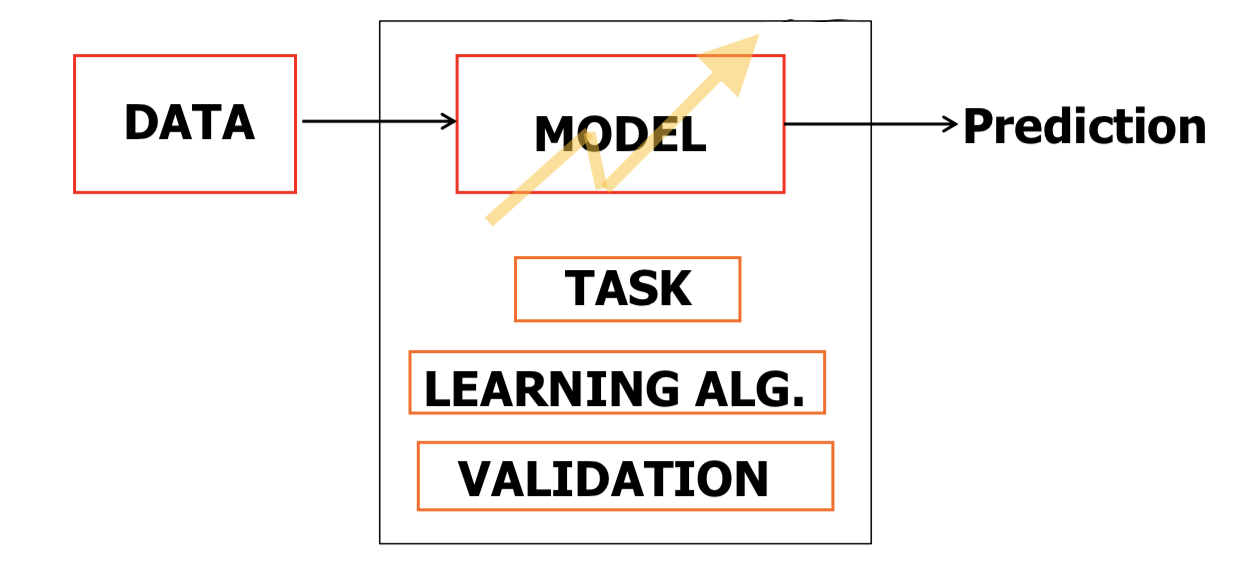
\includegraphics[scale=0.5]{Images/modelloML.png}
\end{figure}

\begin{itemize}
    \item DATA: i dati li ricaviamo dalle osservazioni del mondo
    \item MODEL: i dati passano attraverso un modello. Il modello non è fissato: ha dei parametri liberi, modificabili per fornire le predizioni in modo che siano quelle che vorremmo che fossero fornite.
    \begin{itemize}
        \item TASK: Supervised o Unsupervised Learning
        \item LEARNING ALGORITHM: algoritmo che cerca la soluzione in uno spazio di stati
        \item VALIDATION: valutazione statistica del modello (quanto riesce ad essere accuratosui dati futuri). 
    \end{itemize}
    \item PREDICTION: è l'output restituito dal modello
\end{itemize} 
"Apprendere" viene visto come una approssimazione di una funzione sconosciuta ricavata dagli esempi. 

\subsubsection{Riconoscimento caratteri}
Un esempio "pilota" che possiamo fare è il riconoscimento di caratteri scritti a mano. Il problema è racchiuso nel riconoscere una funzione che passa per un insieme di punti. Come input abbiamo una collezione di immagini di caratteri scritti a mano. Il problema è costruire un modello che riceve in input queste matrici di 8x8 pixel e come output restituire la cifra riconosciuta.
\begin{figure}[H]
    \centering
    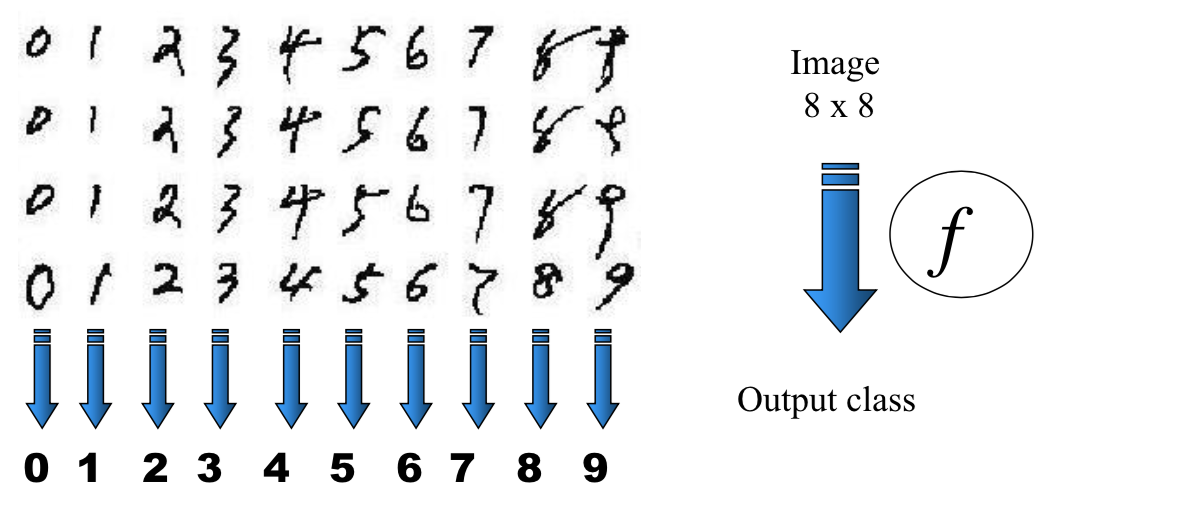
\includegraphics[scale=0.5]{Images/caratteririconoscimento.png}
\end{figure}
Non sappiamo quale sia la funzione, perché in quel caso la scriveremmo direttamente in un algoritmo. Cerchiamo quindi di approssima una funzione facendo restituire come output una classificazione della matrice di pixel. Il problema di classificazione è dato dalla formalizzazione della soluzione esatta, poiché ci possiamo trovare con dati rumorosi o ambigui. Risulta però facile raccogliere collezioni di esempi etichettati, cioè esempi con soluzioni associate. \newline
Generalizzando il problema possiamo usare la tecnica del Supervised Learning. In particolare abbiamo in input uno spazio x di dati etichettati, dobbiamo costruire una funzione generale a partire dagli esempi e come output dare una categoria o valori reali. 

\subsection{TASK: Supervised Learning}
Il Supervised Learnin è una tecnica di apprendimento automatico che mira a istruire un sistema informatico in modo da consentirgli di elaborare automaticamente previsioni sui valori di uscita di un sistema rispetto ad un input sulla base di una serie di esempi ideali, costituiti da coppie di input e di output, che gli vengono inizialmente forniti. \newline
Quindi vengono dati esempi di training nella forma di coppie $<input,output>$ = $<x,d>$ (esempi etichettati) per la creazione di una funzione sconosciuta f. Definiamo il valore target come il valore "d" che vogliamo ottenere come output (e che ci viene dato tramite gli esempi). \newline
Bisogna trovare una buona approssimazione di f, cioè una ipotesi h che può essere usata per predire l'output sui dati sconosciuti x'. \newline
L'obiettivo è dare in output una etichetta numerica o la classificazione del dato. 
\begin{itemize}
    \item Classificazione: la funzione a valori discreti f(x) restituisce la presunta classe corretta per x.
    \item Regressione: consiste nell'approssimare a valori reali la funzione target.
\end{itemize}
Entrambi sono compiti di approssimazione di funzione.

\subsection{TASK: UNsupervised Learning}
L'apprendimento non supervisionato è una tecnica di apprendimento automatico che consiste nel fornire al sistema informatico una serie di input (esperienza del sistema) che egli riclassificherà ed organizzerà sulla base di caratteristiche comuni per cercare di effettuare ragionamenti e previsioni sugli input successivi. Abbiamo quindi un TR set che è un insieme di dati non etichettati, il compito è quello di raggruppare i dati in insiemi consistenti. I principali algoritmi sono:
\begin{itemize}
    \item Clustering: raggruppamento di elementi omogenei in un insieme di dati (cluster) identificando un centroide.
    \item Dimensionality reduction / Visualization / Preprocessing
    \item Modeling the data density
\end{itemize}
\begin{figure}[H]
    \centering
    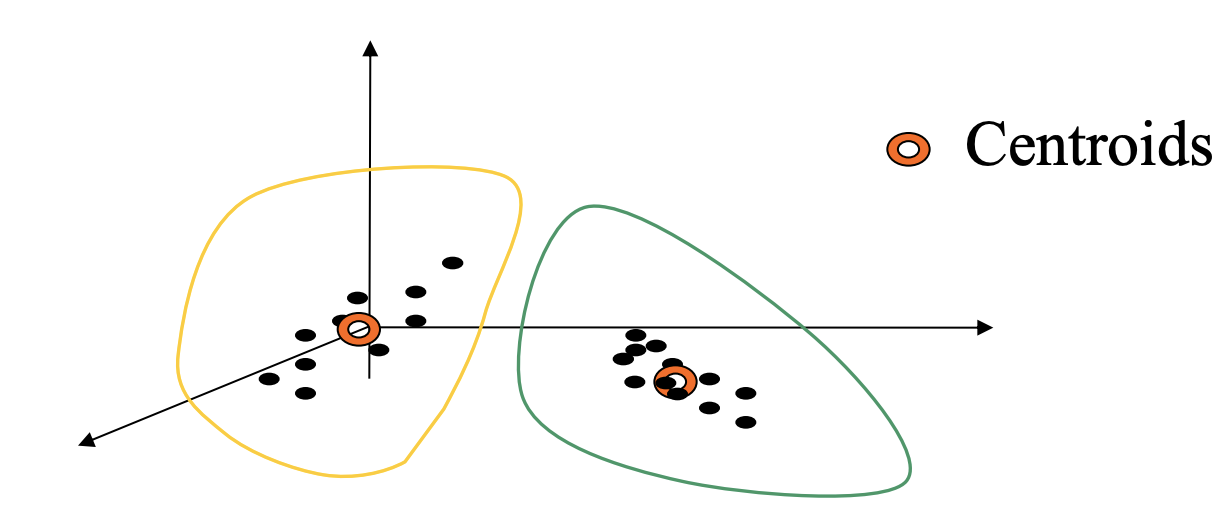
\includegraphics[scale=0.4]{Images/clustering.png}
    \caption{Esempio di clustering}
\end{figure}

\subsection{MODEL}
Il compito è quello di catturare e descrivere le relazioni tra i dati sulla base del TASK. Il modello definisce la classe delle funzioni che la macchina può implementare (cioé definisce lo spazio delle ipotesi). \newline
Concetti utili: 
\begin{itemize}
    \item Training examples: fanno parte del Supervised Learning ed é un insieme di esempi nella forma (x,f(x)) dove x è un vettore di caratteristiche e f(x) è il valore obiettivo.
    \item Target function: la funzione obiettivo f il piú possibile corretta
    \item Hypotesis: è una funzione h che è ritenuta di essere simile a f. La funzione h è data in un linguaggio capace di esprimere le relazioni tra i dati.
    \item Hypoteses space: è lo spazio di tutte le ipotesi che possono essere output dell'algoritmo. É dove cerchiamo la funzione h. 
\end{itemize}
I linguaggi per le ipotesi h devono saper esprimere modelli di ML: ad esempio la logica del primo ordine, equazioni numeriche oppure calcolo delle probabilità.

\subsubsection{Esempi di Modelli}
\begin{itemize}
    \item Modelli Lineari: la rappresentazione di H definisce uno spazio continuo parametrizzato di potenziali ipotesi. Come parametro abbiamo w, ed ogni assegnamento di w è una ipotesi differente. (es: $h_w(x)=w_1x+w_0$)
    \item Regole simboliche: lo spazio delle ipotesi è basato su rappresentazioni discrete, sono possibili differenti regole come ad esempio: if ($x_1$=0 and $x_2$=1) then h(x)=1 else h(x)=0
    \item Modelli probabilistici: stimare p(x,y)
    \item Approcci basati sull'istanza: confronta le nuove istanze del problema con le istanze osservate durante l'addestramento, che sono state memorizzate. Si chiama basato sull'istanza perché costruisce ipotesi direttamente dalle istanze di addestramento stesse.
\end{itemize}

\subsection{LEARNING ALGORITHM}
Gli algoritmi di apprendimento si basano su DATA, TASK e MODEL. L'euristica consiste nella ricerca delle migliori ipotesi nello spazio delle ipotesi H, cioè la miglior approssimazione della funzione obiettivo f sconosciuta (ad esempio i parametri liberi del modello vengono adattati al compito da svolgere: il miglior w nel modello lineare, la miglior regola per regole simboliche, ecc...). H potrebbe non coincidere con l'insieme di tutte le possibili funzioni e la ricerca può non risultare esaustiva, per questo bisogna fare assunzioni (vedremo in seguito il ruolo dell'Inductive Bias).
\begin{figure}[H]
    \centering
    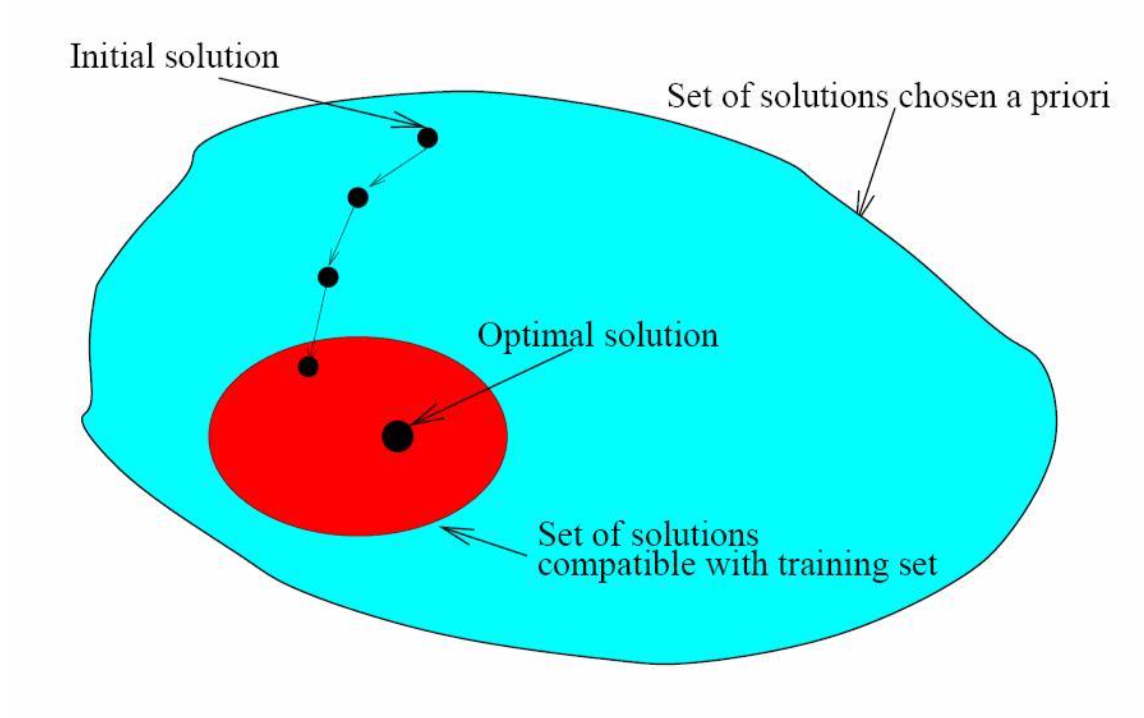
\includegraphics[scale=0.4]{Images/learningalgo.png}
\end{figure}

\subsection{VALIDATION - Generalizzazione}
L'apprendimento può essere quindi definito come la ricerca una buona funzione, in uno spazio di funzioni restituito da dati conosciuti. "Buona funzione" considerando l'errore di generalizzazione (o capacità di generalizzazione) cioè quanto accuratamente il modello prevede nuovi campioni di dati. La generalizzazione è cruciale in ML $\rightarrow$ strumenti corretti di ML.
\begin{itemize}
    \item Fase di apprendimento (training, fitting): costruire il modello dai dati di training conosciuti (Training Set).
    \item Fase predittiva (test): si applica la funzione costruita a un nuovo esempio. Si prende in input x, si computa la risposta dal modello e confrontiamo l'output con il nostro target (che il modello non ha mai visto). Si esegue una valutazione dell'ipotesi predittiva, ad esempio la valutazione della capacità di generalizzazione (valutazione statistica del modello, quanto riesce ad essere accurato sui dati futuri). É bene notare che essere performanti in ML significa predire accuratamente, cioé la performance é stimata dagli errori effettuati calcolando la funzione sul Test Set (che é diverso dal Training set!).
\end{itemize}

\section{Concept Learning}
Il Concept Learning anche noto come apprendimento di categoria é definito come "la ricerca di attributi che possono essere utilizzati per distinguere i modelli dai non modelli di varie categorie". Più semplicemente, i concetti sono le categorie che ci aiutano a classificare oggetti, eventi o idee, basandoci sul fatto che ogni oggetto, evento o idea ha un insieme di caratteristiche rilevanti comuni. In un compito di Concept Learning, una macchina viene addestrata per classificare gli oggetti mostrandole una serie di oggetti di esempio insieme alle loro etichette di classe. La macchina semplifica ciò che ha osservato "condensandolo" sotto forma di un esempio. Questa versione semplificata di ciò che è stato appreso viene quindi applicata a esempi futuri. \newline
Lavoriamo in uno spazio discreto strutturato come lo spazio delle ipotesi, useremo come rappresentazione la congiunzione di letterali e vedremo algoritmi come Find-S ed Candidate Elimination. Praticamente in questa sezione andremo ad vedere in cosa consiste la classificazione del Supervised Learning, cioé come la funzione f(x) restituisce la presunta classe corretta per x.

\begin{quote}
    Concept Learning: dedurre una funzione booleana (con dominio X e codominio \{t,f\}) da esempi di allenamento positivi e negativi (dove X é lo spazio che contiene le istanze)
\end{quote}
Un Training example é definito come coppia <x,c(x)> (le coppie sono contenute nel Training Set). \newline
L'ipotesi h:$X \rightarrow {0,1}$ soddisfa x se h(x)=1. \newline
Una ipotesi h é consistente con un esempio di allenamento <x,c(x)> se h(x)=c(x) con x appartenete a X. É consistente anche con D\footnote{é sempre il Training Set insieme degli esempi} se h(x)=c(x) per ogni esempio di allenamento <x,c(x)> in D.

\subsubsection{Esempio: Apprendimento Funzione Booleana}
\begin{figure}[H]
    \centering
    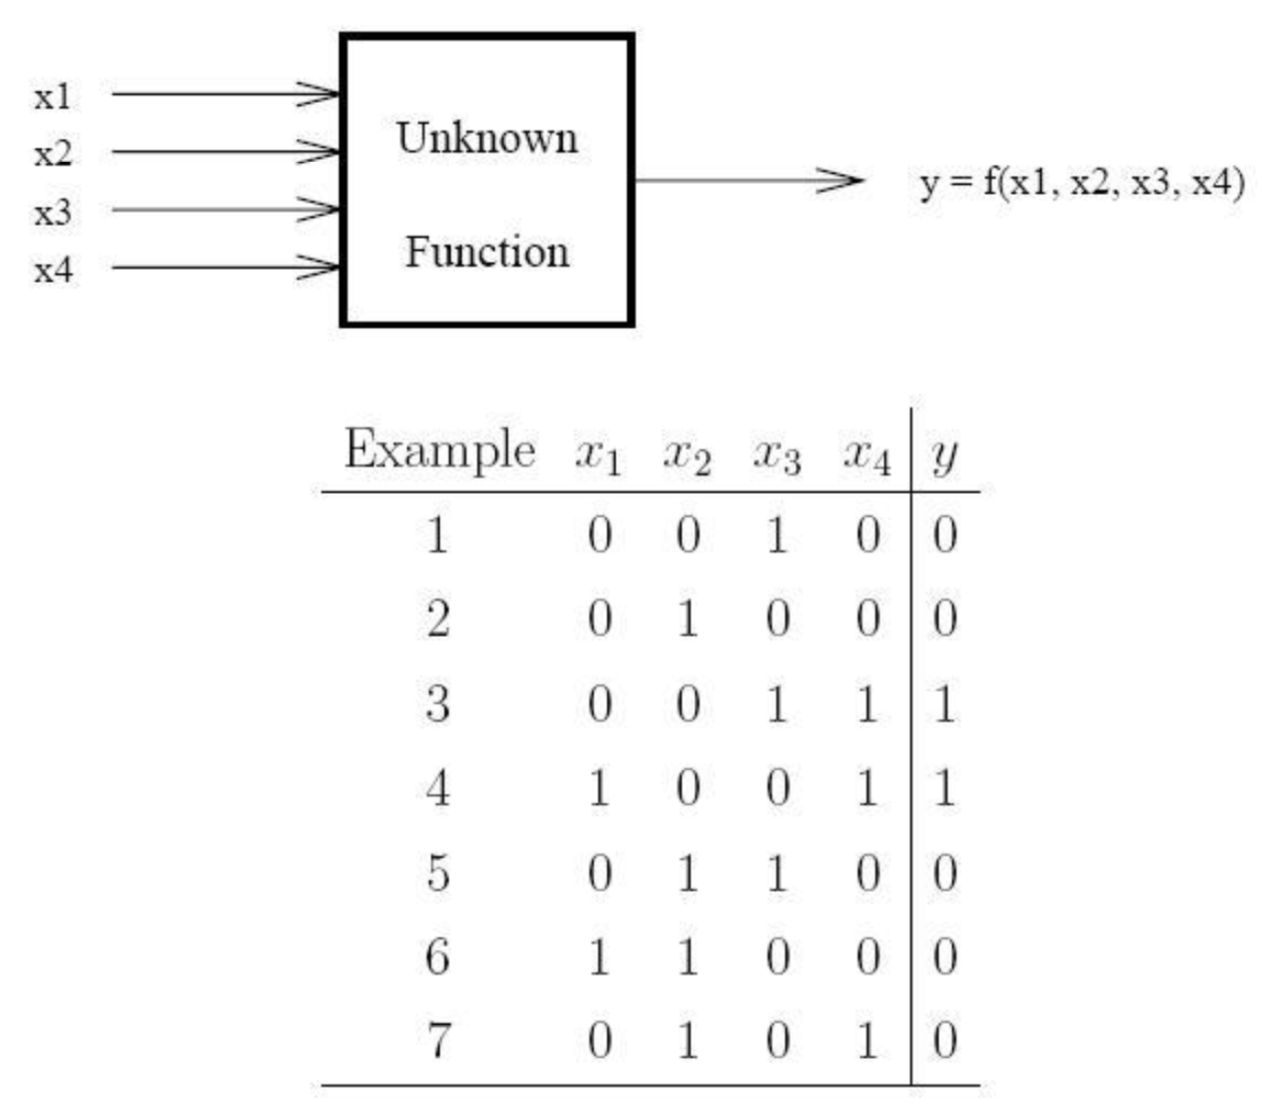
\includegraphics[scale=0.4]{Images/esempiofunzionebooleana.png}
\end{figure}
Questo é un problema mal posto poiché potremmo violare l'esistenza, unicità o stabilità della soluzione. Come possiamo vedere dall'immagine abbiamo in input 4 variabili e in output un singolo valore. Nella tabella troviamo il nostro training set (D) e il nostro compito é quello di trovare la funzione che dati in input quei valori restiutisce l'output definito dalla tabella. Ci sono $2^{2^4}$ possibili funzioni booleane per 4 ingressi, questo perché abbiamo $2^4$ possibili ingressi e per ognuno possiamo rispondere 0 o 1. Non possiamo sapere quale sia la funzione corretta fino a che non abbiamo visto tutte le possibili coppie di input/output. Dopo aver analizzato i nostri 7 esempi ci rimangono ancora $2^9$ possibilità. Nel caso generale per input/output binari la formula é $|H| = 2^{numeroistanze} = 2^{2^n}$ dove $|H|$ é la dimensione dello spazio delle ipotesi ed n é la dimensione dell'input. \newline
Lavoreremo con uno spazio delle ipotesi ristretto: partiamo scegliendo uno spazio delle ipotesi H che é considerevolmente più piccolo dello spazio di tutte le possibili funzioni. Vedremo: 
\begin{itemize}
    \item proposizioni formate da solo "and" (regole congiuntive) in uno spazio di ipotesi H finito e discreto
    \item funzioni lineari, in uno spazio di ipotesi H continuo e infinito
\end{itemize}

\subsection{Regole Congiuntive}
Quante h diverse possiamo avere? Cioè quante semplici regole congiuntive? \newline
Nel caso generale:
\begin{itemize}
    \item Letterali positivi: ad esempio $h_1 = l_2$, $h_2=(l_1 \land l_2)$, $h_3 = true$ ecc... sono semplici regole congiuntive. Abbiamo ridotto lo spazio delle ipotesi così da ottenere $|H| = 2^n$ basti immaginare $l_i$ come una stringa di bit di lunghezza n.
    \item Letterali: (di cui fa parte anche il not($l_i$) ottenendo uno spazio delle ipotesi di dimensione $3^n+1$
\end{itemize}
Vedremo come organizzare e cercare in modo efficiente attraverso uno spazio di ipotesi, sfruttando algoritmi per un insieme di ipotesi molto limitato semplificandoci il lavoro usando dati non rumorosi.

\subsection{Problema: Enjoy Sport}
Concept: "giorni in cui piace fare sport acquatici" \newline
Task: predire il valore di "Enjoy Sport" per un giorno arbitrario in base ai valori degli attributi.
\begin{table}[H]
\centering
\begin{tabular}{l|l|l|l|l|l|l}
Sky & Temp & Humid & Wind & Water & Forecast & Enjoy Sport? \\ \hline
Sunny & Warm & Normal & Strong & Warm & Same & Yes \\
Sunny & Warm & High & Strong & Warm & Same & Yes \\
Rainy & Cold & High & Strong & Warm & Change & No \\
Sunny & Warm & High & Strong & Cool & Change & Yes
\end{tabular}
\end{table}
Una riga della tabella é una istanza.

\subsection{Rappresentare le Ipotesi}
L'ipotesi h é una congiunzione di vincoli sugli attributi. Ogni vincolo può essere:
\begin{itemize}
    \item Uno specifico valore: ad esempio Water = Warm
    \item Un valore irrilevante: ad esempio Water = ?
    \item Nessun valore consentito (ipotesi nulla): ad esempio Water = 0
\end{itemize}
Esempio di ipotesi h:
\begin{table}[H]
\centering
\begin{tabular}{l|l|l|l|l|l}
Sky & Temp & Humid & Wind & Water & Forecast \\ \hline
Sunny & ? & ? & Strong & ? & Same
\end{tabular}
\end{table}
corrispondente alla funzione booleana
\begin{quote}
    $Sky=Sunny \land Wind=Strong \land Forecast=Same$
\end{quote}
L'ipotesi più specifica (risponde sempre false) e più generale (risponde sempre true) sono rispettivamente
\begin{table}[H]
\centering
\begin{tabular}{l|l|l|l|l|l}
Sky & Temp & Humid & Wind & Water & Forecast \\ \hline
0 & 0 & 0 & 0 & 0 & 0 \quad //specifica \\
? & ? & ? & ? & ? & ? \quad //generale
\end{tabular}
\end{table}

\subsection{TASK del Concept Learning}
Vengono dati:
\begin{itemize}
    \item Le istanze X: i possibili giorni vengono descritti da attributi Sky, Temp, Humid, Wind, Water e Forecast.
    \item Funzione Target: c:EnjoySport $X \rightarrow{0,1}$.
    \item Spazio delle ipotesi (H): insieme finito di coniunzioni di letterali
    \item Esempi di allenamento (D): esempi positivi e negativi: $<x_1, c(x_1)>, ..., <x_n, c(x_n)>$
\end{itemize}
Bisogna trovare:
\begin{itemize}
    \item Una ipotesi h in H tale che h(x)=c(x) per tutti gli x in X
\end{itemize}
L'apprendimento sta nella ricerca nello spazio delle ipotesi H.

\subsection{Apprendimento Induttivo}
\begin{quote}
    Assunzione: "Qualsiasi ipotesi trovata per approssimare la funzione target sugli esempi di allenamento, approssimerà anche la funzione target sugli esempi non osservati". Non è detto che il Training Set sia corretto (dati rumorosi, ...)
\end{quote}
Quindi h(x)=c(x) per ogni x in D (funzione consistente con il training set) ma h(x)=c(x) per ogni x in X? Problema fondamentale del ML.

\subsection{Qual é il numero di istanze, concetti e ipotesi di un problema?}
\begin{itemize}
    \item Sky: Sunny, Cloudy, Rainy
    \item Temp: Warm, Cold
    \item Humid: Normal, High
    \item Wind: Strong, Weak
    \item Water: Warm, Cold
    \item Forecast: Same, Change
\end{itemize}
La scelta della rappresentazione di H determina lo spazio di ricerca! \newline
Numero di possibili istanze: 3*2*2*2*2*2 = 96 \newline
Numero di concetti distinti: $2^96 = 2^{numeroistanze}$ \newline
Numero di ipotesi sintatticamente distinte: 5*4*4*4*4*4 (poiché per ogni attributo devo aggiungere 0 o ?) \newline
Numero di ipotesi semanticamente distinte: 1+4*3*3*3*3*3 (poiché le ipotesi con almeno uno 0 sono equivalenti a false, i valori sono in and!) \newline
Strutturare uno spazio di ricerca può aiutare a cercare in modo piú efficiente.

\subsection{Da ordine generale a ordine specifico}
Consideriamo due ipotesi
\begin{enumerate}
    \item $h_1$ = $<Sunny,?,?,Strong,?,?>$
    \item $h_2$ = $<Sunny,?,?,?,?,?>$
\end{enumerate}
L'insieme di istanze coperte da $h_1$ e da $h_2$ sono differenti, infatti $h_2$ impone meno vincoli rispetto a $h_1$ e quindi classifica più istanze x positive (h(x)=1).
\begin{quote}
    Siano $h_j$ e $h_k$ funzioni booleane definite su X. $h_j$ é più generale o equivalente a $h_k$ ($h_j \geq h_k$) se solo se $\forall x \in X : [(h_k(x)=1) \rightarrow (h_j(x)=1)$
\end{quote}
Un esempio sulle ipotesi binarie: $l_1 \geq (l_1 \land l_2)$ non sono comparabili, la relazione $\geq$ impone un ordine parziale sullo spazio delle ipotesi H. Possiamo sfruttare questo ordine parziale per organizzare più efficientemente la nostra ricerca in H.
\begin{figure}[H]
    \centering
    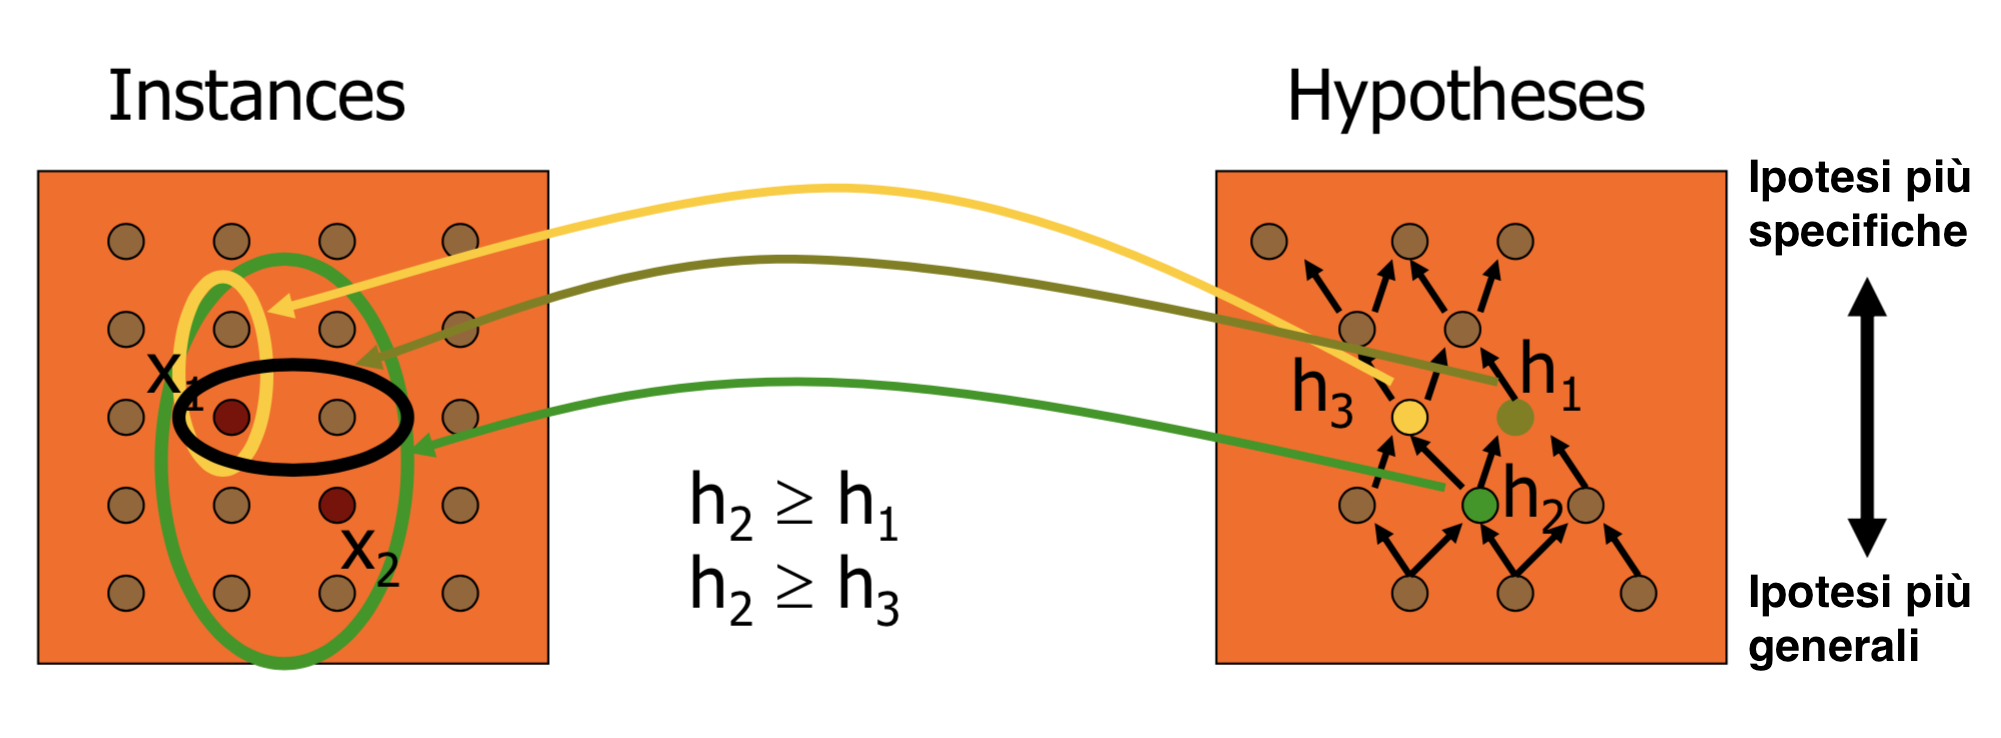
\includegraphics[scale=0.4]{Images/partialorder.png}
    \caption{Partial Order}
\end{figure}
Istanze:
\begin{itemize}
    \item $x_1$ = $<Sunny,Warm,High,Strong,Cool,Same>$
    \item $x_2$ = $<Sunny,Warm,High,Light,Warm,Same>$
\end{itemize}
Ipotesi:
\begin{itemize}
    \item $h_1$ = $<Sunny,?,?,Strong,?,?>$
    \item $h_2$ = $<Sunny,?,?,?,?,?>$
    \item $h_3$ = $<Sunny,?,?,?,Cool,?>$
\end{itemize}

\subsection{Algoritmo Find-S (Specific)}
L'algoritmo Find-S sfrutta l'ordine parziale di gestione per cercare in modo efficiente una h consistente (senza elencare esplicitamente ogni h in H).
\begin{enumerate}
    \item Inizializza h con l'ipotesi più specifica nello spazio delle ipotesi H ($h_0 = <0, 0, 0, 0, 0, 0>$)
    \item Prendo il prossimo esempio di training:
        \begin{itemize}
            \item Per ogni attributo $a_i$ dell'ipotesi h, se $a_i$ é soddisfatto in h da x allora non fare nulla (quindi se l'esempio é negativo non ci sono cambiamenti sull'ipotesi), altrimenti se $a_i$ NON é soddisfatto e l'esempio é positivo, sostituisci $a_i$ con il prossimo vincolo più generale soddisfatto da x. \newline 
            Ripeto il passaggio per ogni esempio positivo.
        \end{itemize}
    \item Viene dato in output l'ipotesi h
\end{enumerate}
L'algoritmo parte dall'ipotesi più specifica, poi scende in maniera conservativa (generalizza il minimo possibile) in modo da rimanere consistente sui positivi, e di conseguenza contemporaneamente sui negativi. Trovo un'ipotesi che copre tutti i positivi e tutti i negativi. In questo modo evito di esplorare tutto H, scorrendo solo una volta il training set, perché si segue il Partial Order.
\subsubsection{Esempio su Enjoy Sport}
\begin{enumerate}
    \item $h_0 = <0, 0, 0, 0, 0, 0>$
    \item $x_1 = <Sunny, Warm, Normal, Strong, Warm, Same>$ \quad questo esempio é positivo\footnote{l'esempio é preso dalla tabella a pagina 9} e $h_0$ non é soddisfatta perché False. Quindi devo prendere i vincoli più generali da $x_1$ e metterli in h, in questo caso sono le singole istanze poiché tutte piú generali di 0.
    \item $h_1 = <Sunny, Warm, Normal, Strong, Warm, Same>$
    \item $x_2 = <Sunny, Warm, \textcolor{red}{High}, Strong, Warm, Same>$ \quad esempio positivo, notiamo che High é in constrasto con Normal. Quindi cambio quell'attributo con uno piú generale, in questo caso é "?".
    \item $h_2 = <Sunny, Warm, ?, Strong, Warm, Same>$
    \item $x_3 = <Rainy, Cold, High, Strong, Warm, Change>$ \quad esempio é negativo quindi non faccio nulla
    \item $h_3 = <Sunny, Warm, ?, Strong, Warm, Same>$
    \item $x_4 = <Sunny, Warm, High, Strong, \textcolor{red}{Cool}, \textcolor{red}{Change}>$ \quad esempio positivo
    \item $h_3 = <Sunny, Warm, ?, Strong, ?, ?>$
\end{enumerate}

\subsubsection{Proprietà di Find-S}
Lo spazio delle ipotesi é rappresentato come congiunzione di attributi (molto limitativo), l'algoritmo darà in output l'ipotesi più specifica, nello spazio H, che é consistente con gli esempi positivi del training set. L'ipotesi di output h sarà anche consistente con gli esempi negativi, a condizione che il concetto target sia contenuto in H.
\subsubsection{Aspetti negativi di Find-S}
Non so se il sistema di apprendimento converga con il concetto target, nel senso che non è in grado di determinare se ha trovato l'unica ipotesi coerente con gli esempi di allenamento. Inoltre non so quando i dati di allenamento sono incoerenti, in quanto ignora gli esempi di allenamento negativi $\rightarrow$ nessuna tolleranza al rumore sui dati!

\subsection{Version Spaces}
Find-S fornisce una ipotesi da H che è coerente con gli esempi di allenamento, questa è solo una delle tante ipotesi da H che potrebbero adattarsi ugualmente bene ai dati di allenamento. L'idea é quindi quella di dare in output l'insieme di tutte le possibili h consistenti con D.
\begin{quote}
    Il Version Space $VS_{H,D}$ rispetto allo spazio delle ipotesi H e il training set D, é il sottoinsieme delle ipotesi prese da h coerenti con tutti gli esempi di training: $VS_{H,D} = {h \in H | Consistent(h,D) }$ dove $Consistent(h,D) = \forall<x,c(x)> \in D | h(x)=c(x)$
\end{quote}
Si dice che un esempio x soddisfa l'ipotesi h quando h(x) = 1, indipendentemente dal fatto che x sia un esempio positivo o negativo del concetto target. Tuttavia, se un tale esempio sia coerente con h dipende dal concetto target e, in particolare, se h(x) = c(x).

\subsubsection{Esempio di Version Space }
\begin{figure}[H]
    \centering
    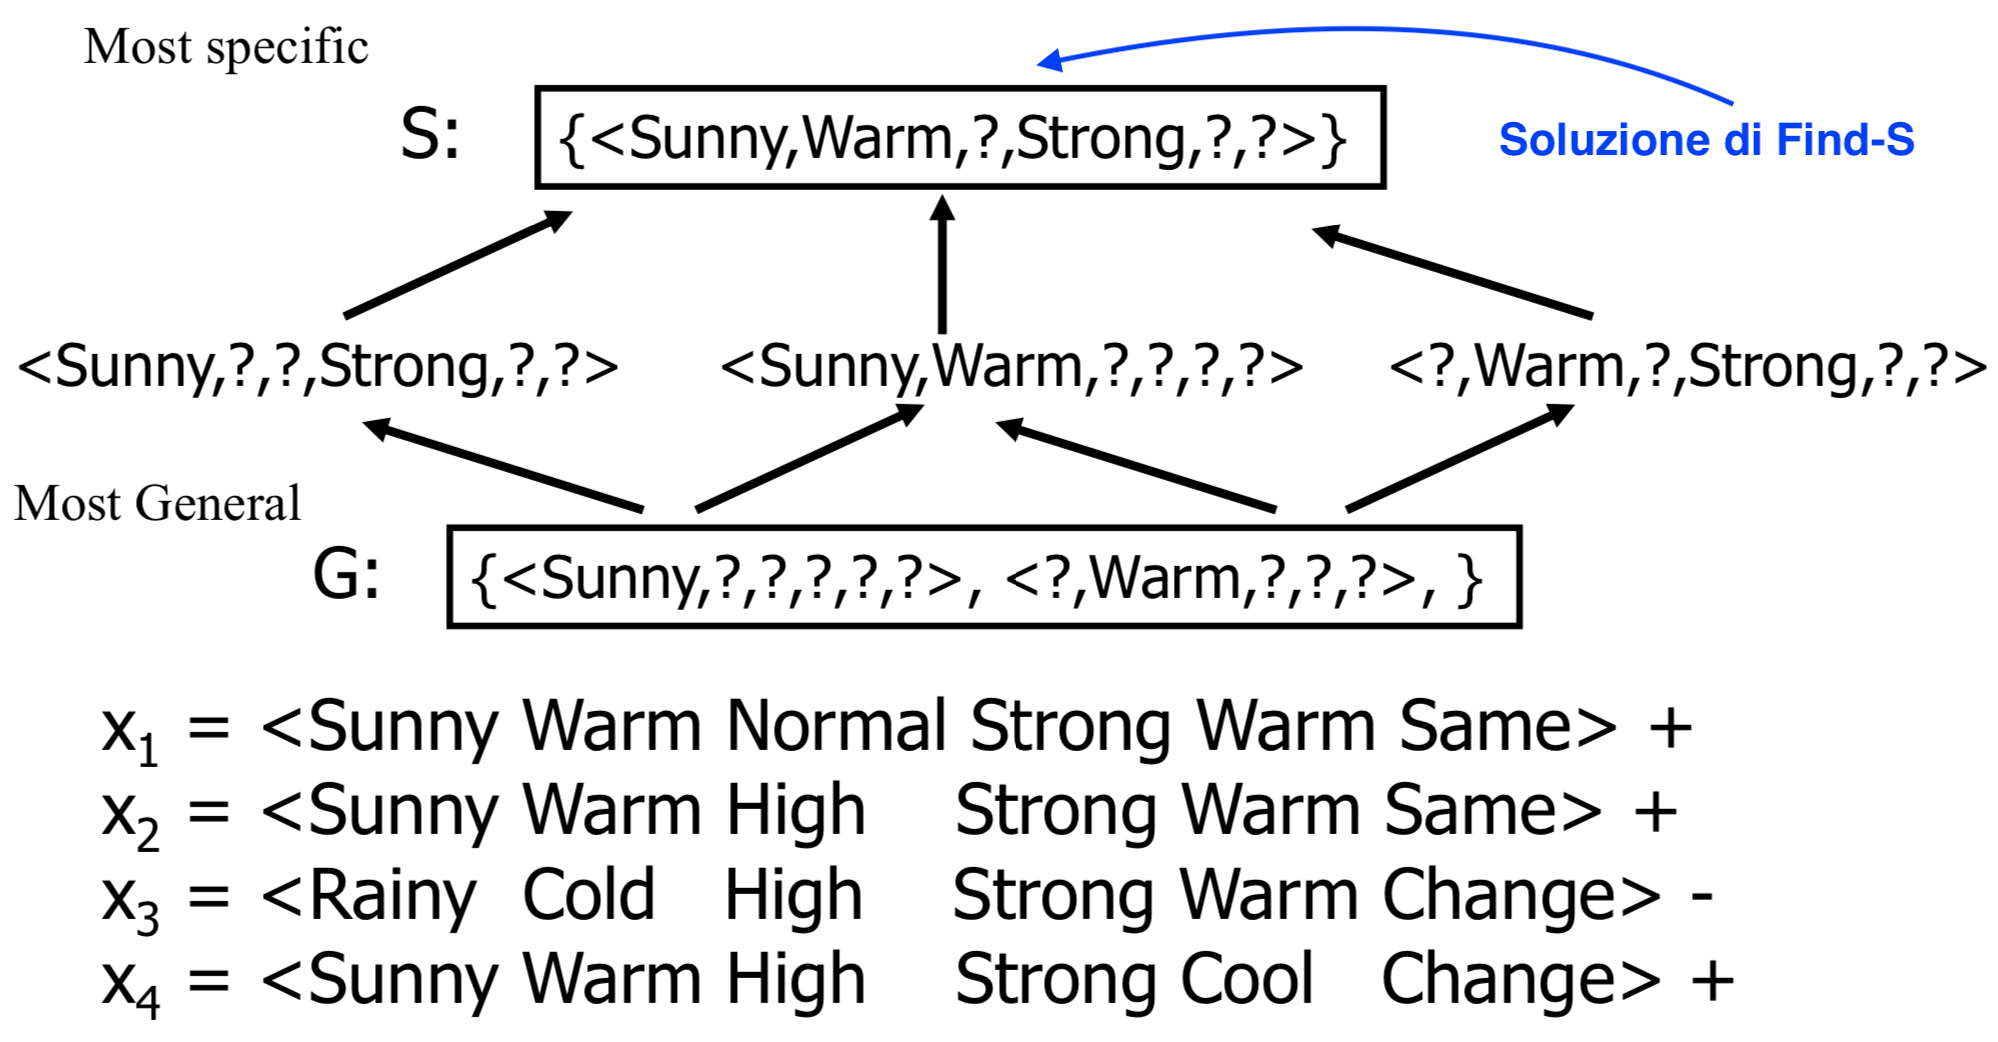
\includegraphics[scale=0.4]{Images/versionspacegs.png}
\end{figure}
Il Version Space dell'algoritmo viene rappresentato solo dal suo membro più generale G e dal più specifico S (che é la soluzione di Find-S!).
\begin{quote}
    Teorema: ogni membro del Version Space si trova tra: $VS_{H,D} = \{h \in H| (\exists s \in S) (\exists g \in G) (g \geq h \geq s)\}$
\end{quote}
dove $x \geq y$ significa x é piú generale o uguale a y. \newline

\subsection{Algoritmo List-Then-Eliminate}
Il Version Space si riduce quindi man mano che si osservano più esempi, fino a quando idealmente rimane solo un'ipotesi coerente con tutti gli esempi osservati, presumibilmente, questo è il concetto target desiderato. Se non sono disponibili dati sufficienti per restringere lo spazio l'algoritmo può generare l'intero insieme di ipotesi coerenti con i dati osservati. L'algoritmo List-Then-Eliminate può essere applicato ogni volta che lo spazio di ipotesi H è finito. Ha molti vantaggi, tra cui il fatto che è garantito il risultato di tutte le ipotesi coerenti con i dati di allenamento. Sfortunatamente, richiede un elenco esaustivo di tutte le ipotesi in H, un requisito non realistico per tutti gli spazi di ipotesi tranne quelli più banali.
\begin{enumerate}
    \item Iniziamo impostando il nostro Version Space con una lista contente ogni ipotesi in H
    \item Per ogni esempio di allenamento $<x,c(x)>$ rimuoviamo dal Version Space ogni ipotesi che é inconsistente con gli esempi di allenamento cioé $h(x)!\neq(x)$
    \item Viene dato in output la lista delle ipotesi ora contenute nel Version Space
\end{enumerate}

\subsection{Algoritmo Candidate Elimination}
L'algoritmo di Candidate Elimination calcola il Version Space contenente tutte le ipotesi di H che sono coerenti con una sequenza osservata di esempi di addestramento. L'algoritmo di eliminazione dei candidati calcola la descrizione di questo set senza elencare esplicitamente tutti i suoi membri. Ciò si ottiene utilizzando l'ordinamento più generale che parziale e mantenendo una rappresentazione compatta dell'insieme di ipotesi coerenti. \newline
Inizia inizializzando il Version Space sull'insieme di tutte le ipotesi in H, cioè inizializzando il set di limiti G per contenere l'ipotesi più generale in H $G_0 = <?, ?, ?, ?, ?, ?>$ e inizializzando il set di limiti S per contenere l'ipotesi più specifica $S_0 = <0, 0, 0, 0, 0, 0>$. Questi due insiemi di limiti delimitano l'intero spazio delle ipotesi, poiché ogni altra ipotesi in H è sia più generale di $S_0$ sia più specifica di $G_0$. Dopo che tutti gli esempi sono stati elaborati, lo spazio versione calcolato contiene tutte le ipotesi coerenti con questi esempi.
\begin{enumerate}
    \item Inizializza G con l'insieme di ipotesi massimamente generali in H $G_0 = <?, ?, ?, ?, ?, ?>$
    \item Inizializza S con l'insieme di ipotesi massimamente specifiche in H $S_0 = <0, 0, 0, 0, 0, 0>$
    \item Per ogni esempio di training $d=<x,c(x)>$:
        \begin{itemize}
            \item se d é positivo: 
                \begin{itemize}
                    \item Rimuovere da G ogni ipotesi incompatibile con d
                    \item per ogni ipotesi s in S che non è coerente con d: (Generalizziamo S)
                        \begin{itemize}
                        \item Rimuovere s da S
                        \item Aggiungi a S tutte le minime generalizzazioni h di s tali che h é consistente con d e alcuni membri di G sono più generali di h
                        \item Rimuovi da S ogni ipotesi più generale di un'altra ipotesi in S
                        \end{itemize}
                \end{itemize}
            \item se d é negativo: 
                \begin{itemize}
                    \item Rimuovere da S ogni ipotesi incompatibile con d
                    \item per ogni ipotesi g in G che non è coerente con d: (Specializziamo G)
                        \begin{itemize}
                        \item Rimuovere g da G
                        \item Aggiungi a G tutte le minime specializzazioni h di g tali che h é consistente con d e alcuni membri di S sono più specifici di h
                        \item Rimuovi da G ogni ipotesi meno generale di un'altra ipotesi in G
                        \end{itemize}
                \end{itemize}
        \end{itemize}
\end{enumerate}

\subsubsection{Esempio di Candidate Elimination}
\begin{figure}[H]
    \centering
    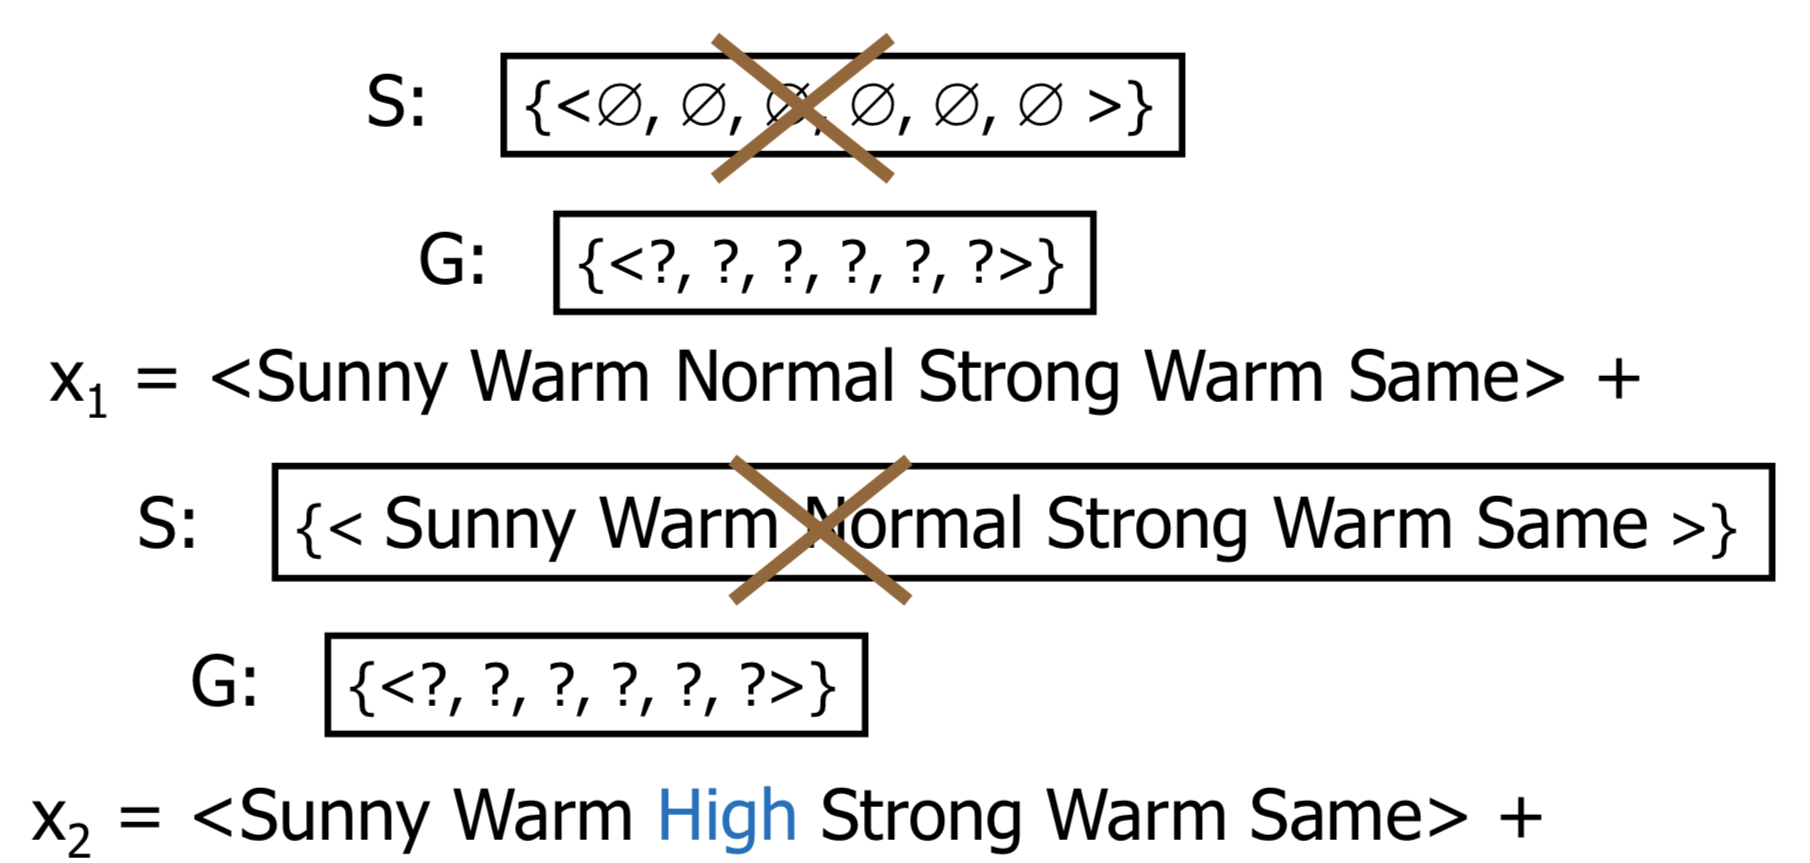
\includegraphics[scale=0.4]{Images/candidateelim1.png}
    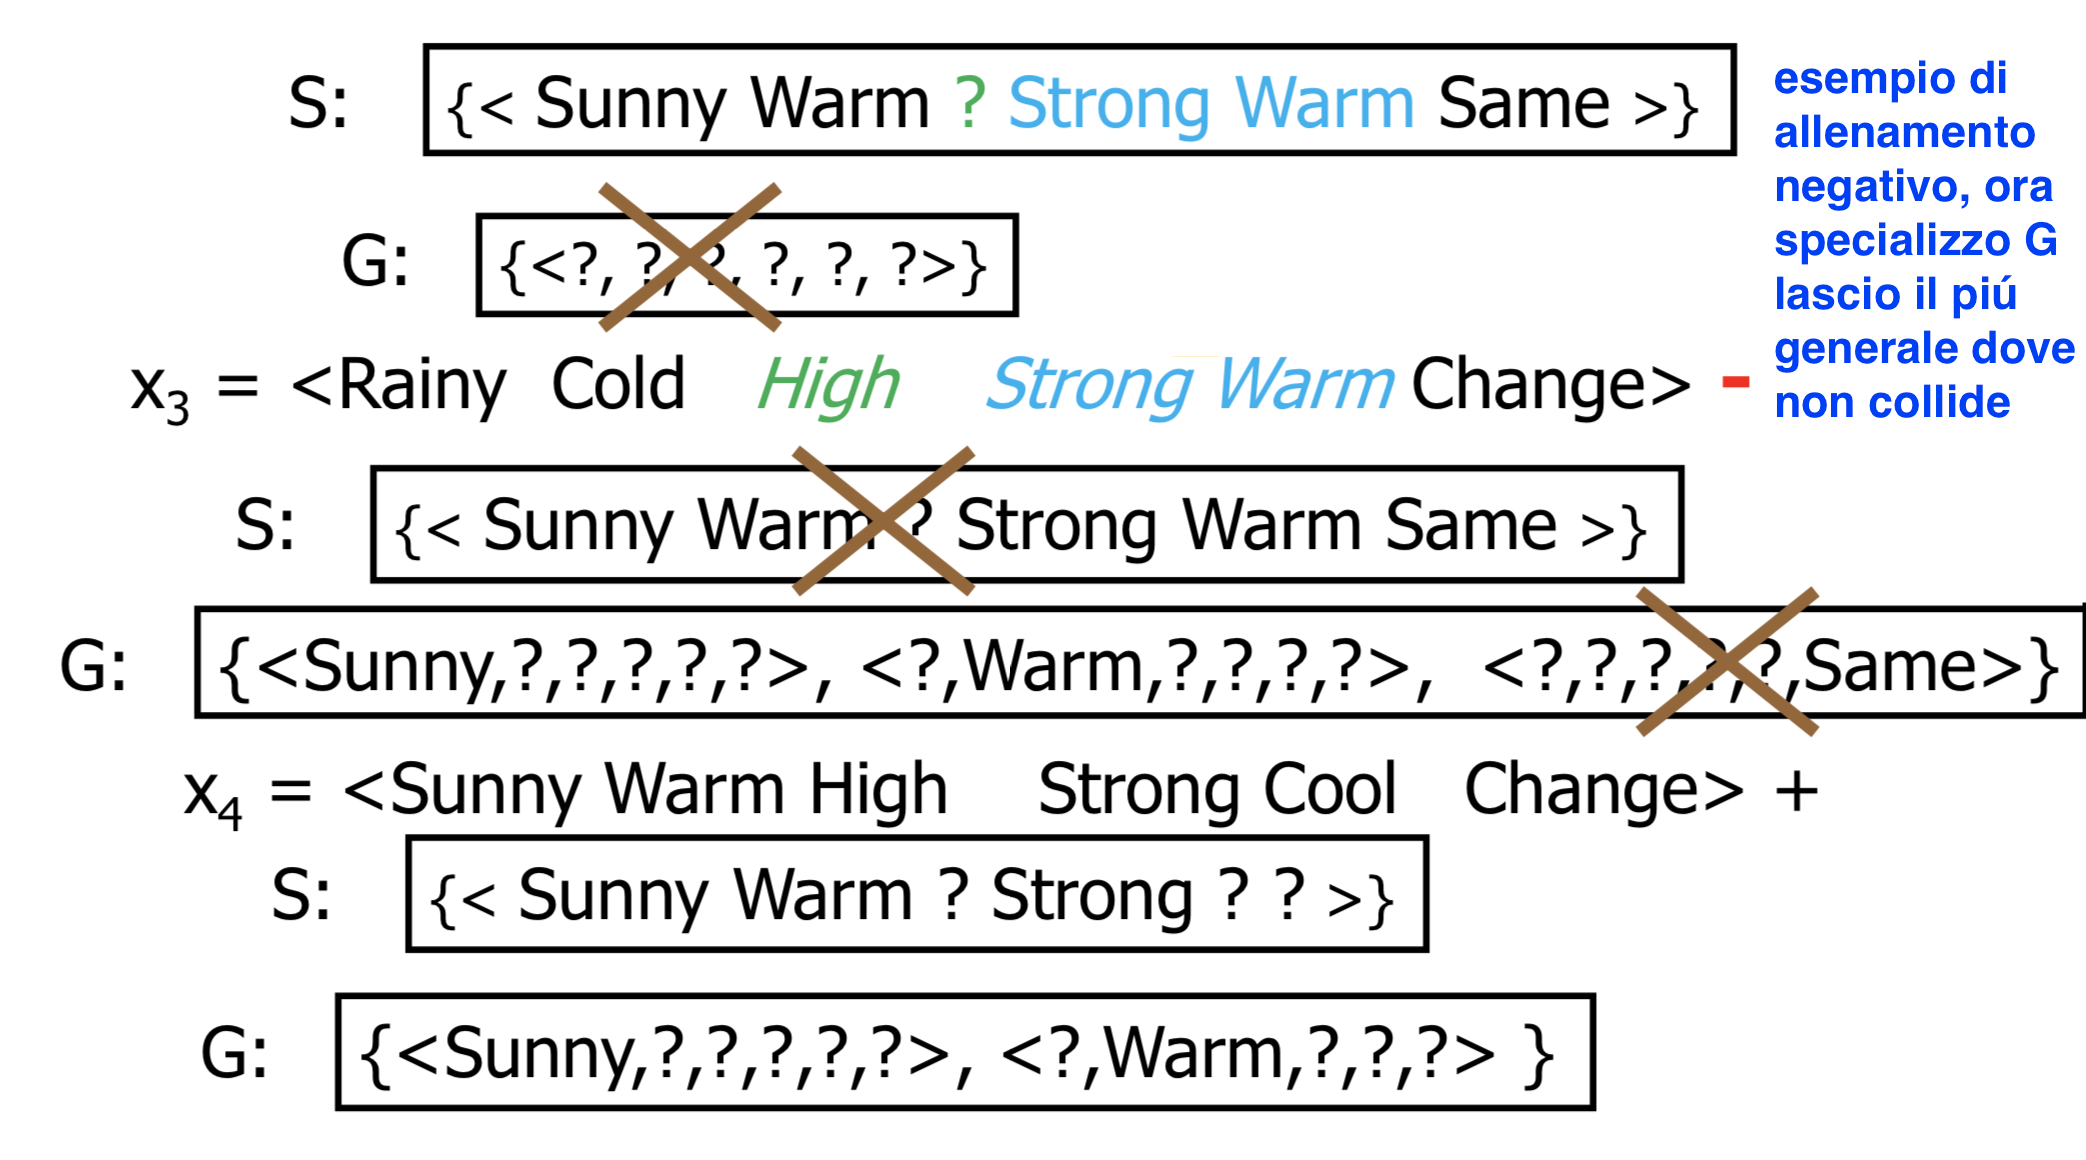
\includegraphics[scale=0.4]{Images/candidateelim2.png}
\end{figure}
G al passaggio 3 contiene le specializzazioni minime che mi permettono di coprire $x_3$ come negativa, senza rendere G più specializzato di S. S e G sono le "guardie" di tutti i positivi e di tutti i negativi trovati finora. Il fatto che se specializzo troppo G rendo false alcuni input già accettati, deriva dal partial order: intelligentemente il controllo di consistenza di tutti i vecchi input non è effettuato dall'algoritmo. Infatti, il limite S del Version Space costituisce un riepilogo degli esempi positivi riscontrati in precedenza che possono essere utilizzati per determinare se una ipotesi è coerente con questi esempi. Il limite G riassume le informazioni da esempi negativi riscontrati in precedenza. Ogni ipotesi più specifica di G è garantita per essere coerente con esempi negativi del passato.

\section{Inductive Bias}
Il nostro spazio delle ipotesi non é in grado di rappresentare target disgiuntivi come ad esempio $(Sky=Sunny) \lor (Sky=Cloudy)$. \newline
Se avessimo due esempi del tipo: \newline
$x_1 = <Sunny, Warm, Normal, Strong, Cool, Change>$ (positivo) \newline
$x_2 = <Cloudy, Warm, Normal, Strong, Cool, Change>$ (positivo) \newline
troveremo che $S = \{ <?, Warm, Normal, Strong, Cool, Change> \}$ \newline
che é inconsistente con l'esempio $x_3 = <Rainy, Warm, Normal, Strong, Cool, Change >$ (negativo) \newline
trovando $S = \{\}$, cioé S collassa, perché la funzione target è fatta solo di and \newline
PROBLEMA: abbiamo vincolato il sistema di apprendimento considerando solo ipotesi congiuntive. Abbiamo bisogno di uno spazio di ipotesi più espressivo. Supponiamo che lo spazio delle ipotesi H contenga il concetto target c. In altre parole, che c può essere descritta da una congiunzione di letterali.

\subsection{Sistema di apprendimento Unbiased}
La ovvia soluzione al problema di assicurare che il concetto target sia nello spazio di ipotesi H è di fornire uno spazio di ipotesi in grado di rappresentare ogni concetto insegnabile. \newline
Significa che H è l'insieme di tutti i possibili sottoinsiemi di X: l'insieme di potenza P(X). In EnjoySport $|H|=96$, $|P(X)|=2^96$ concetti distinti. Un'ipotesi può essere rappresentata con disgiunzioni, congiunzioni e negazioni delle nostre precedenti ipotesi. H sicuramente contiene il concetto target. Con questa modifica quali sono i nostri G e S? \newline
NUOVO PROBLEMA: il nostro algoritmo di apprendimento dei concetti non è ora in grado di generalizzare oltre gli esempi osservati. Assumiamo tre esempi positivi $(x_l, x_2, x_3)$ e due esempi negativi $(x_4, x_5)$. $S = \{(x_1 \lor x_2 \lor x_3) \}$ e $G = \{\neg (x_4 \lor x_5)\}$ $\rightarrow$ Non abbiamo generalizzazione! Gli unici esempi classificati in modo non ambiguo sono gli stessi esempi di addestramento.
\begin{quote}
    Proprietà: un sistema di apprendimento imparziale non è in grado di generalizzare \newline
    Prova: ogni istanza non osservata verrà classificata positivamente precisamente da metà delle ipotesi in Version Space e negativa dell'altra metà. Infatti $\forall h$ consistente con $x_i(test)$, $\exists h'$ identico ad h con eccezione che $h'(x_i) \neq h(x_i)$ cioé $h \in VS \rightarrow h' \in VS$ (sono identici in D)
\end{quote}

\subsubsection{Il learning Unbiased é utile?}
Un sistema di apprendimento che non fa assunzioni preliminari riguardo all'identità del concetto target non ha basi razionali per classificare eventuali istanze non conosciute. Uno sistema di apprendimento dovrebbe essere in grado di generalizzare i dati di allenamento usando presupposti precedenti al fine di classificare istanze invisibili. La generalizzazione è nota come salto induttivo e le nostre assunzioni precedenti sono il vincolo induttivo del sistema di apprendimento. Il bias non è solo assunto per efficienza, ma è necessario per la generalizzazione, tuttavia non ci dice quale sia la migliore soluzione per la generalizzazione. \newline
\subsection{Definizione Formale di Inductive Bias}
Consideriamo:
\begin{itemize}
    \item Un algoritmo di apprendimento concettuale L
    \item Un insieme di istanze X e un concetto target c
    \item Sia $D_c = \{<x, c(x)>\}$ un insieme di esempi di training di c
    \item Sia $L(x_i, D_c)$ la classificazione assegnata all'istanza $x_i$ da L dopo l'allenamento su $D_c$.
\end{itemize}
\begin{quote}
    L'Inductive Bias di L è un insieme minimo di asserzioni B tale che per qualsiasi concetto target c e corrispondenti dati di allenamento $D_c$: \newline
    $(\forall x_i \in X)[B \land D_c \land x_i] \vdash L(x_i,D_c)$ dove $A \vdash B$ significa che B é deducibile da A.
\end{quote}

\subsection{Sistemi Induttivi e Deduttivi equivalenti}
\begin{figure}[H]
    \centering
    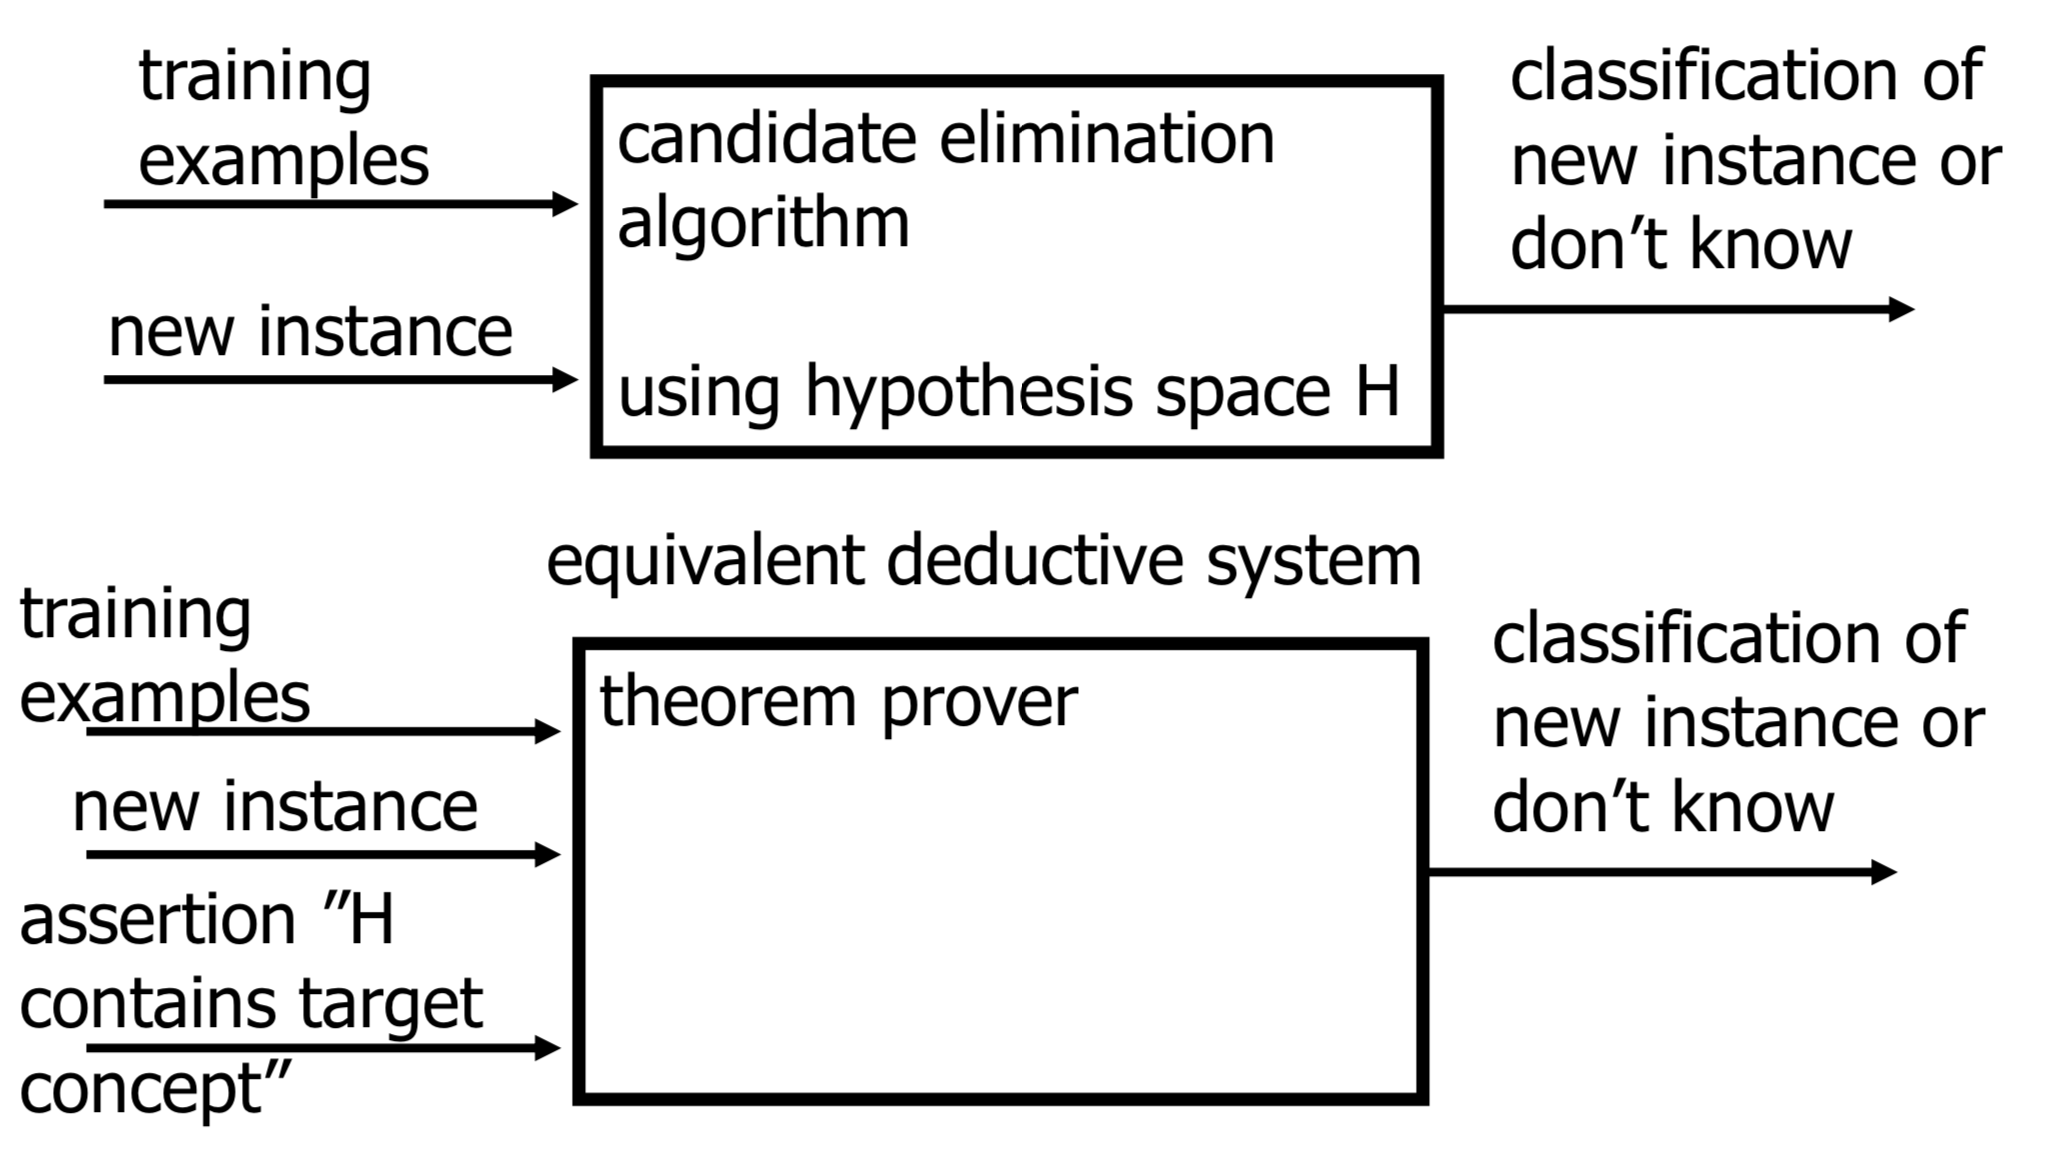
\includegraphics[scale=0.4]{Images/sistemiinduttdedutt.png}
\end{figure}
Il Bias è l'insieme delle asserzioni che ci permette di trasformare il problema da induttivo a deduttivo.
\subsection{Tre (algoritmi) sistemi di apprendimento con Bias differenti}
\begin{enumerate}
    \item Rote Learner: (lookup table) L'apprendimento corrisponde semplicemente alla memorizzazione di ogni esempio di allenamento osservato nella memoria. Le istanze successive vengono classificate osservandole nella memoria. Se l'istanza viene trovata in memoria, viene restituita la classificazione memorizzata. In caso contrario, il sistema rifiuta di classificare la nuova istanza. In poche parole salva gli esempi, classifica x se e solo se si "accoppiano" con uno degli esempi visti precedentemente. \newline 
    Non c'è Bias Induttivo $\rightarrow$ nessuna generalizzazione
    \item Candidate Elimination: Le nuove istanze vengono classificate solo nel caso in cui tutti i membri del Version Space corrente concordino la classificazione. In caso contrario, il sistema rifiuta di classificare la nuova istanza. \newline 
    Bias Induttivo $\rightarrow$ il concetto target può essere rappresentato nel suo spazio di ipotesi. 
    \item Find-S: Questo algoritmo, descritto in precedenza, trova l'ipotesi più specifica coerente con gli esempi di addestramento. Quindi utilizza questa ipotesi per classificare tutte le istanze successive. \newline
    Bias Induttivo $\rightarrow$ il concetto target può essere rappresentato nel suo spazio delle ipotesi e tutte le istanze sono istanze negative a meno che l'opposto non sia implicato da altre sue conoscenze.
\end{enumerate}

%fin qui ok

\section{Modelli Lineari}
Sintesi:
\begin{itemize}
    \item Dati di Allenamento
    \item Spazio delle Ipotesi H: costituisce l’insieme delle funzioni che possono essere realizzate dal sistema di apprendimento, si assume che la funzione da apprendere f possa essere rappresentata da una ipotesi h in H (selezione di h attraverso i dati di apprendimento) o che almeno una ipotesi h in H sia simile a f (approssimazione);
    \item Algoritmo di Ricerca nello Spazio delle Ipotesi, algoritmo di apprendimento, ad esempio adattamento dei parametri liberi del modello al task
    \item NOTA: H non puó coincidere con l’insieme di tutte le funzioni possibili e la ricerca essere esaustiva $\rightarrow$ Bias Induttivo
\end{itemize}
Sia la regressione lineare che la classificazione (vista nel Concept Learning) appartengono alla categoria delle tecniche di apprendimento supervisionato, ovvero un tipo di apprendimento che fornisce a priori una serie di dati e informazioni al sistema, prima che questo cominci ad apprendere. La regressione lineare si differenzia nettamente dalla classificazione, poiché quest'ultima si limita a discriminare gli elementi in una determinato numero di classi (label), mentre nella prima l’input è un dato e il sistema ci restituisce un output reale approssimando una funzione. La regressione è un processo statistico che cerca di stabilire una relazione tra due o più variabili. Fornito a un modello di regressione un valore x, questo restituirà il corrispondente valore y generato dall'elaborazione di x.

\subsection{Esempio di regressione}
La regressione come abbiamo detto é un processo di stima di una funzione di valore reale sulla base di una serie finita di campioni rumorosi (conosciamo le coppie (x , f(x)+random noise).
\begin{figure}[H]
    \centering
    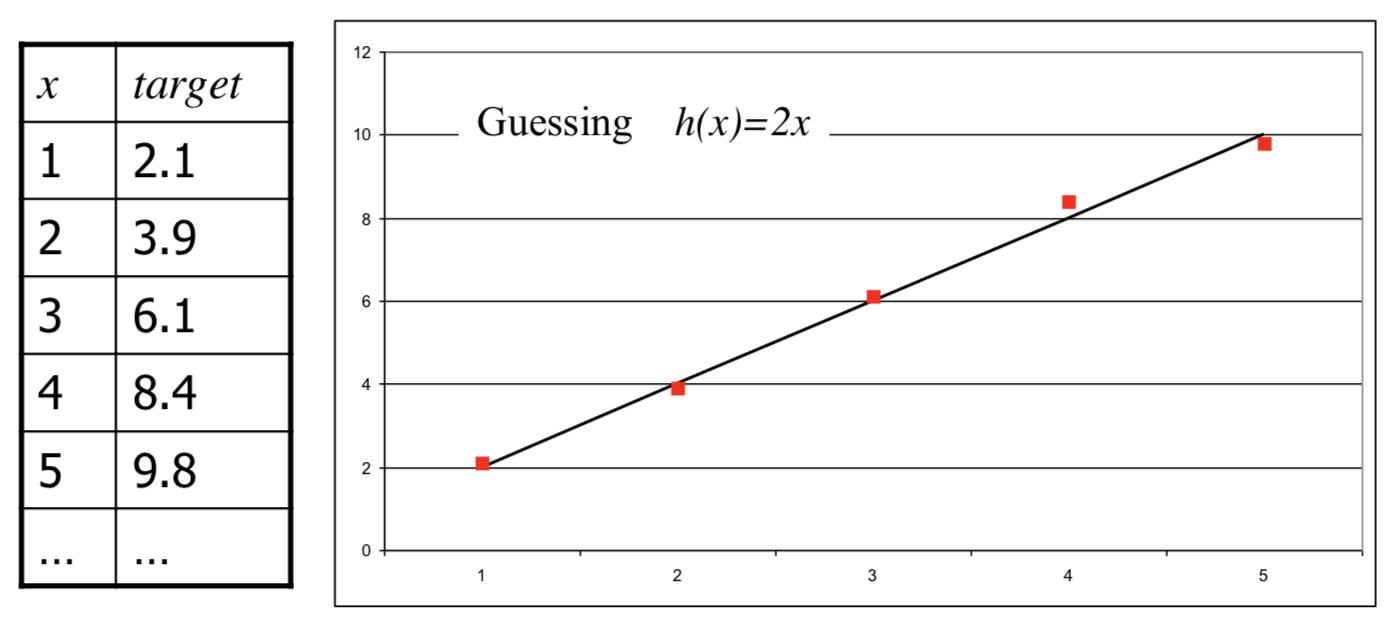
\includegraphics[scale=0.4]{Images/esempioregressione.png}
\end{figure}

\subsection{Modello di regressione lineare semplice}
\begin{quote}
    Si parte con una variabile input x e una in output y, assumiamo il modello $h_w(x)$ espresso come $out=w_1x+w_0$ dove $w_i$ sono parametri liberi a valori reali. Come si può intuire cerchiamo di adattarci ai dati con una linea retta.
\end{quote}
Lavoriamo in uno spazio di ipotesi infinite (i valori w sono continui) ma abbiamo una buona soluzione grazie alla matematica classica, possiamo "imparare" con questo strumento di base. Sebbene semplice, include molti concetti pertinenti della moderna ML ed è una base di metodi evoluti utilizzati nel settore. \newline
Supponendo che la variabile y sia (linearmente) correlata a un'altra variabile (x) o ad altre variabili per cui $y = w_1x + w_0 + noise$, dove i w sono i parametri liberi. "noise" è l'errore nella misurazione degli obiettivi (con distribuzione normale). Cerchiamo di costruire un modello (trovare le variabili $w_i$) per predire/stimare la y per dei valori x non visti precedentemente.
\begin{figure}[H]
    \centering
    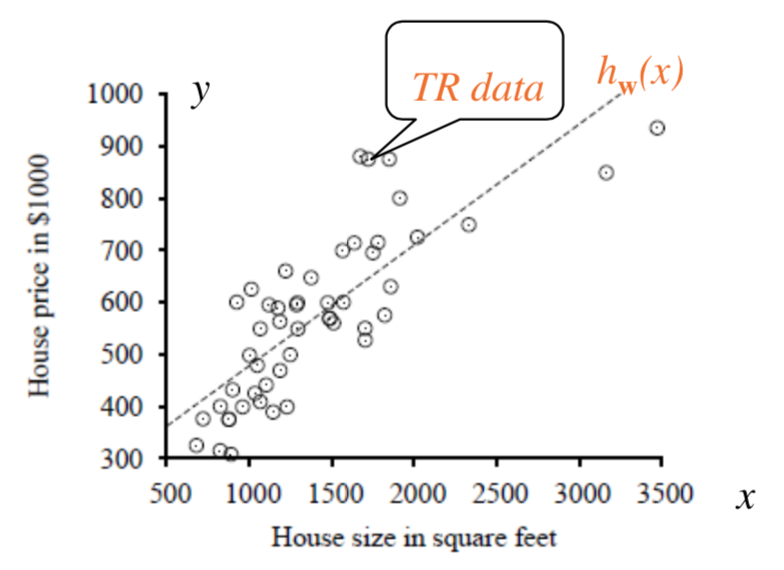
\includegraphics[scale=0.4]{Images/regresslincase1.png}
    \caption{esempio che associa il prezzo delle case in base alla metratura. (y costo della casa, x metratura)}
\end{figure}
Un esempio di regressione lineare per l'esempio sovrastante é la funzione $h_w(x)=0.232*x+246$ ma come arrivare a questa funzione?
\subsection{Costruzione della funzione via LMS}
L'algoritmo LeastMeanSquare consiste nel trovare gli w per minimizzare l'errore (miglior adattamento dei dati sul training set con l esempi).
\begin{itemize}
    \item Dato un insieme di l esempi di allenamento ($x_p,y_p$)
    \item Trovare $h_w(x)=w_1x+w_0$ che minimizza l'errore medio sul Training Set
    \item Per calcolare la funzione di errore loss usiamo la somma dei quadrati delle differenze tra il valore dato dall'esempio $y_p$ e il valore calcolato dalla funzione $h_w(x)$. Il quadrato serve per avere solo valori positivi (si potrebbe anche usare il valore assoluto, ma è meglio di no, lo vedremo in seguito)
    \item \begin{equation}
        Loss(h_w) = E(w) = \sum_{p = 1}^l (y_p - h_w(x_p))^2 = \sum_{p = 1}^l (y_p - (w_1*x_p + w_0)^2
    \end{equation} dove $x_p$ é il p-esimo input e $y_p$ é il p-esimo output dell'esempio p. Dividendo per l ottengo la media.
\end{itemize}
In modo piú complicato dobbiamo trovare l'argomento minimo w tale che l'errore è minimo in L2 (norma 2, le norme inducono una distanza), a livello grafico lo rappresentiamo cosí: 
\begin{figure}[H]
    \centering
    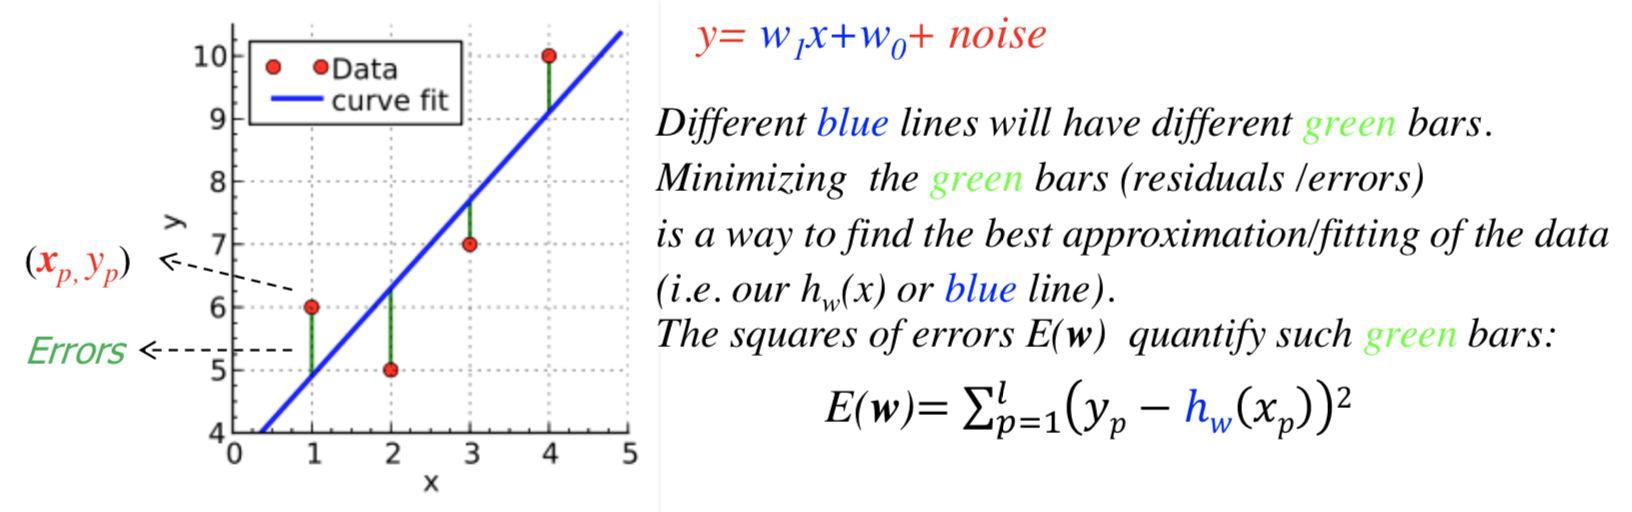
\includegraphics[scale=0.5]{Images/lmsgrafico.png}
\end{figure}
Il metodo dei minimi quadrati è un approccio standard alla soluzione approssimativa di sistemi sovra-determinati, ovvero insiemi di equazioni in cui vi sono più equazioni che incognite. \newline
Il minimo locale é un punto stazionario dove il gradiente é nullo.
\begin{equation}
    \frac{\partial E(w)}{\partial w_i} = 0 \quad per i = 0....dim_space
\end{equation}
per la regressione lineare semplice abbiamo che 
\begin{equation}
    \frac{\partial E(x)}{\partial w_0} = 0 \quad \frac{\partial E(x)}{\partial w_1} = 0
\end{equation}
Se la funzione di perdita é convessa abbiamo la seguente soluzione diretta poiché non abbiamo nessun minimo locale. 
\begin{figure}[H]
    \centering
    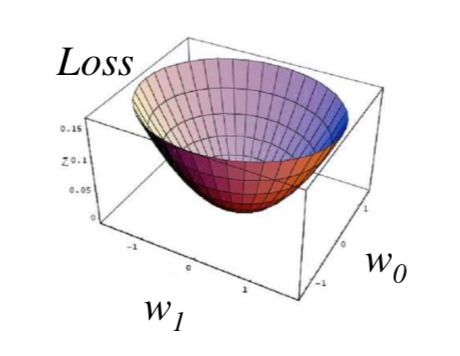
\includegraphics[scale=0.8]{Images/convexlocalmin.png}
\end{figure}

per $w_1$ abbiamo che
\begin{equation}
    w_1 = \frac{\sum x_py_p - \frac{1}{l} \sum x_p \sum y_p}{\sum x_p^2 - \frac{1}{l}(\sum x_p)^2} = 0 = \frac{Cov[x,y])}{Var[x]} 
\end{equation}
mentre per $w_0$
\begin{equation}
    w_0 = \bar{y}-w_1 \bar{x} \quad dove \quad \bar{y}=\frac{1}{l} \sum y_p \quad e \quad \bar{y}=\frac{1}{l} \sum y_p
\end{equation}
Un approccio differente: sfruttiamo le seguenti regole delle derivate parziali per calcolare infine il gradiente

\begin{equation}
   \frac{\partial}{\partial w}k = 0 \quad \frac{\partial}{\partial w}w = 1 \quad \frac{\partial}{\partial w^2}w = 2w \quad \frac{\partial (f(w))^2}{\partial w} = 2f(w) \frac{\partial f(w)}{\partial w}
\end{equation}

ora cerchiamo il gradiente

\begin{equation}
    \frac{\partial E(w)}{\partial w_i} = \frac{\partial (y - h_w(x))^2}{\partial w_i} =  2(y - h_w(x)) \frac{\partial (y - h_w(x))}{\partial w_i} = 2(y - h_w(x)) \frac{\partial (w_1x+w_0)}{\partial w_i}
\end{equation}

sostituendo $w_0$ e $w_1$ nella derivata ottengo due equazioni

\begin{equation}
    \frac{\partial E(w)}{\partial w_0} = -2(y - h_w(x)) \quad e \quad \frac{\partial E(w)}{\partial w_1} = -2(y - h_w(x)) * x
\end{equation}

\begin{figure}[H]
    \centering
    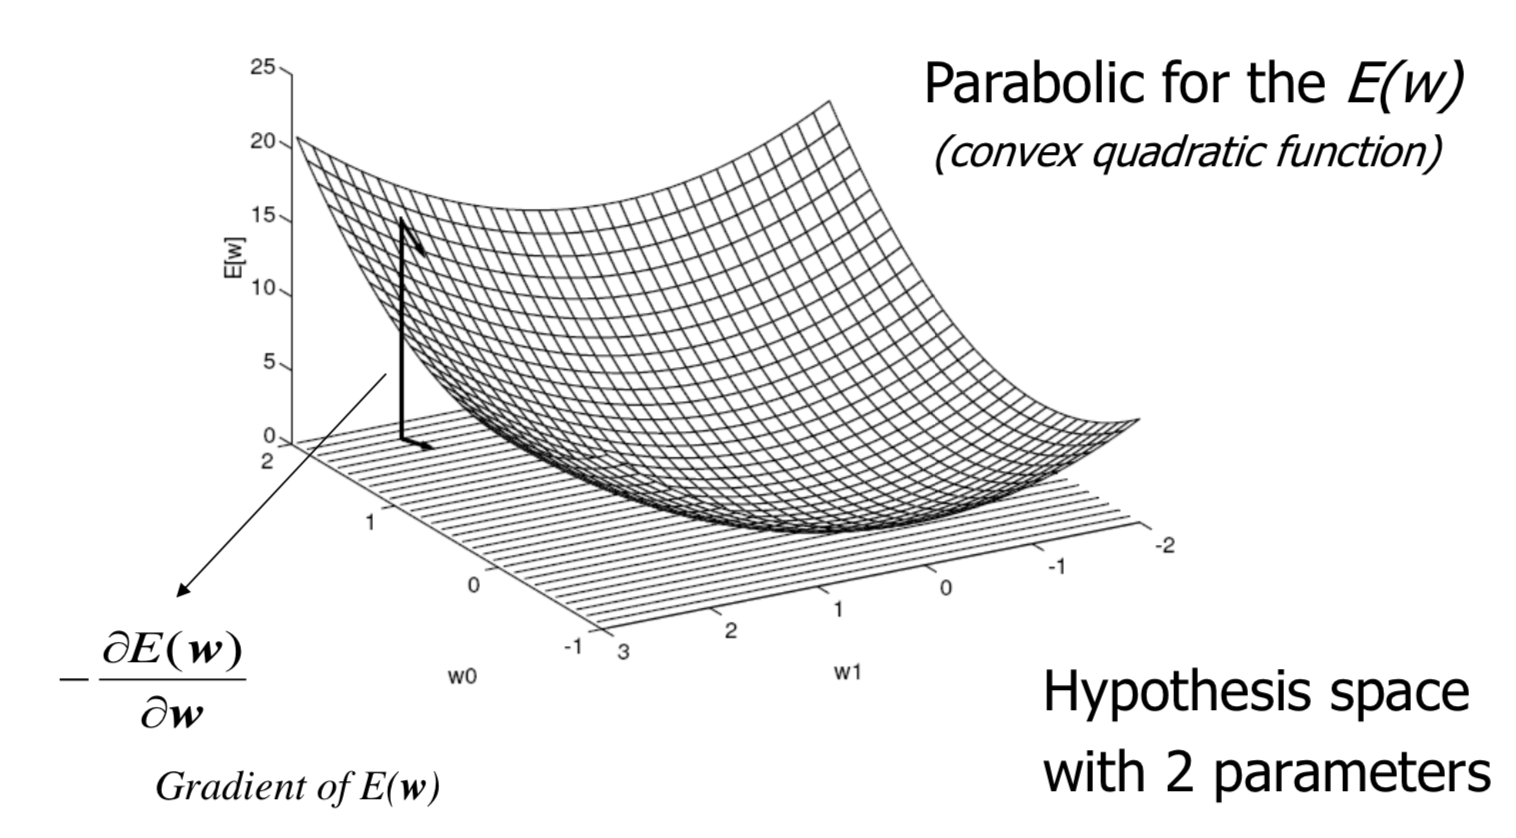
\includegraphics[scale=0.5]{Images/gradientlinearspace.png}
\end{figure}

\subsubsection{Gradiente discendente}
La derivazione precedente suggerisce la costruzione di un algoritmo iterativo basato su $\partial E(w) / \partial w_i$. Il gradiente ci indica la direzione di salita, possiamo spostarci verso il minimo con discesa del gradiente $\Delta w = - gradienteE(w))$. La ricerca locale inizia con il vettore che contiene i valori dei pesi, viene modificato iterativamente per diminuire fino a minimizzare l'errore della funzione.
\begin{quote}
    $w_{new} = w_{old} + \eta * \Delta w$ dove $\eta$ é una costante che indicare il rateo di apprendimento
\end{quote}
\begin{figure}[H]
    \centering
    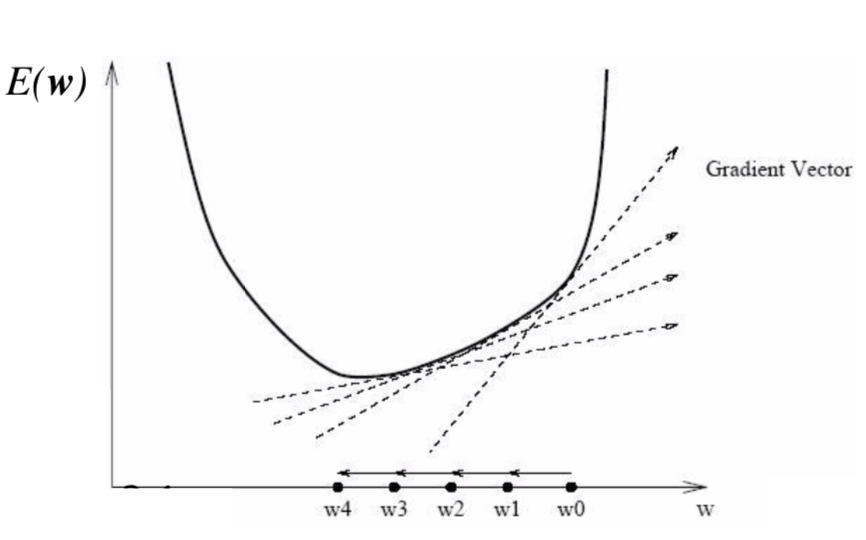
\includegraphics[scale=0.5]{Images/gradientvector.png}
\end{figure}

Le nostre regole di correzione dell'errore (chiamate delta-rule) cambiano i valori w proporzionalmente all'errore:
\begin{equation}
    \Delta w_0 = - \frac{\partial E(w)}{\partial w_0} = 2(y - h_w(x)) \quad e \quad \Delta w_1 = - \frac{\partial E(w)}{\partial w_1} = 2(y - h_w(x)) * x
\end{equation}


\begin{itemize}
    \item se $(y_{target}-output)=0$ significa che non abbiamo errore e quindi nessuna correzione da fare
    \item se $output>y_{target}$ cioé $(y-h)<0$ vuol dire che l'output trovato é troppo alto quindi:
        \begin{itemize}
            \item $\Delta w_0$ negativo $\rightarrow$ riduco $w_0$
            \item se $(x_{input}>0$ $\Delta w_1$ negativo $\rightarrow$ riduco $w_1$ altrimenti incremento $w_1$
        \end{itemize}
    \item se $output<y_{target}$ cioé $(y-h)>0$ vuol dire che l'output trovato é troppo basso quindi:
        \begin{itemize}
            \item $\Delta w_0$ positivo $\rightarrow$ aumento $w_0$
            \item se $(x_{input}>0$ $\Delta w_1$ positivo $\rightarrow$ aumento $w_1$ altrimenti diminuisco $w_1$
        \end{itemize}
\end{itemize}
questo ci permette la ricerca in uno spazio delle ipotesi infinito, e puó essere applicato facilmente per spazi H continui e con perdita differenziabile (? boh) altrimenti non posso calcolare il gradiente. Per questo motivo il valore assoluto è scomodo: potrebbe rendere non differenziabile la funzione. 
arriviamo quindi alle funzioni su l esempi:
\begin{equation}
    \Delta w_0 = - \frac{\partial E(w)}{\partial w_0} = 2 \sum (y_p - h_w(x_p)) \quad e \quad \Delta w_1 = - \frac{\partial E(w)}{\partial w_1} = 2 \sum (y_p - h_w(x_p)) * x_p
\end{equation}
Ora può venirci in mente una domanda, aggiorniamo w dopo un insieme di esempi di allenamento l, oppure dopo ogni esempio analizzato?
\begin{itemize}
    \item Batch Algorithm: Calcoliamo la sommatoria dell’errore quadratico su l pattern diversi e quindi abbiamo il gradiente, dopo l dati di training sommati abbiamo una “epoca” e aggiorniamo la W
    \item On-Line Algorithm: Calcoliamo il gradiente su un pattern p e poi aggiorniamo subito W
\end{itemize}

\subsection{Input Multidimensionali}
Il caso standard é con due variabili ma in realtà possiamo avere in input centinaia di variabili, l'esempio sul prezzo delle case in realtà conteneva anche le variabili che indicavano il numero delle stanze, l'età della casa ecc... 
\subsubsection{Notazione dei dati}
\begin{figure}[H]
    \centering
    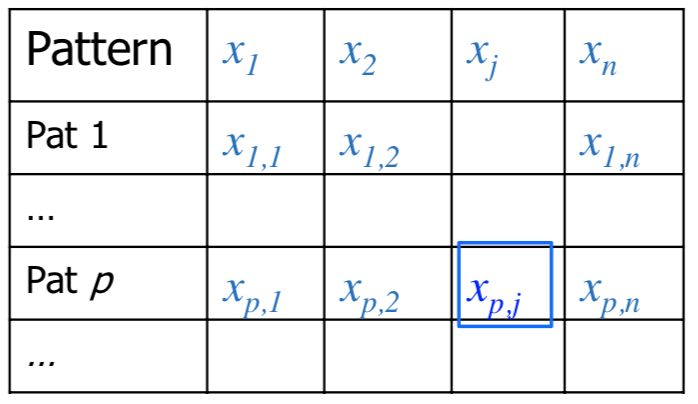
\includegraphics[scale=0.6]{Images/datanotation.png}
\end{figure}
X é una matrice l righe * n colonne (numero di pattern * numero di variabili), ogni riga della matrice $X_i$ é un vettore che rappresenta un esempio. $x_{i,j}$ é uno scalare cioè la componente j della riga i. \newline 
Supponendo vetori colonna x e w, con numero di esempi l e dimensione in input n possiamo scrivere $w^Tx+w_0 = w_0+w_1x_1+w_2x_2+...+w_nx_n$ dove $w_0$ é il bias (non c'entra con il Concept Learning) é la distanza dalla componente 0. Possiamo anche scrivere che $x_0=1$ in modo tale da poter scrivere che $w^Tx = x^Tw$ quindi: $x^T = [1,x_1,...,x_n]$ e $w^T = [w_0, w_1, ..., w_n]$
\subsubsection{Hyperplane}
Anzichè "fittare" una retta, "fittiamo" un iperpiano. 
\begin{figure}[H]
    \centering
    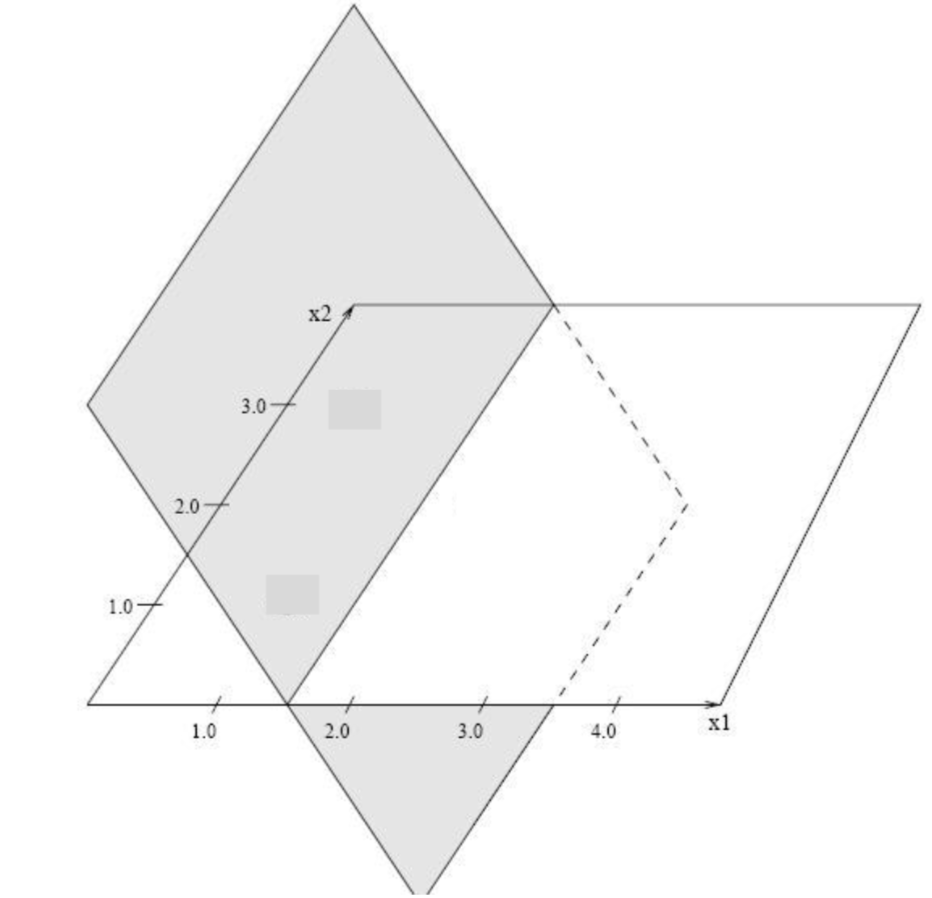
\includegraphics[scale=0.6]{Images/iperpiano.png}
\end{figure}
quindi abbiamo che $w^Tx = w_1x_1 + w_2x_2 + w_0$ e $h(x_p) = x_p^Tw=\sum_{i = 0}^n x_{p,i} w_i$

\subsection{Gradiente Discendente Algoritmo}
\begin{enumerate}
    \item si inizia con il vettore dei pesi $w_{iniziale}$ e si fissa un $0<\eta <1$
    \item si calcola il gradiente $\Delta w = gradienteE(w) = -(\partial E(w) / \partial w)$
    \item si calcola $w_{new} = w_{old} + \eta * \Delta w$
    \item ripetere dal passo 2 finché E(w) é sufficientemente piccolo
\end{enumerate}
La versione batch dell'algoritmo si occupa di calclare $\Delta w$ dopo un insieme di di esempi l. La versione online invece aggiorna $\Delta w$ dopo ogni esempio p al posto di aspettare la sommatoria su l, ma ha bisogno di uno step size $\eta$ piú piccolo. 

\begin{figure}[H]
    \centering
    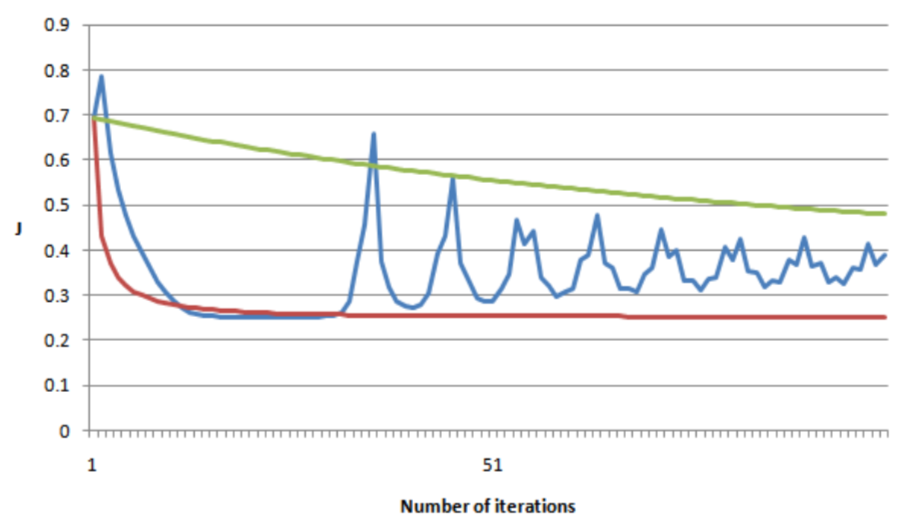
\includegraphics[scale=0.6]{Images/examplegraphloss.png}
\end{figure}

questi sono tre esempi di curve, dove noi andremo a preferire quella che diminuisce nel minor tempo possibile (quella che impiega meno iterazioni). 

\subsection{Vantaggi dei modelli lineari}
Se funziona bene è un modello "meraviglioso", molto semplice dove tutte le informazioni sui dati sono contenute nei w. Facile da interpretare tant'è che viene usato in medicina, biologia, chimica, economia... Una delle cose fondamentali é che sono ammessi dati rumorosi e viene usato/incluso in modelli più complessi.

\subsection{Limitazioni}
La regressione lineare presenta delle limitazioni quando si parla di problemi non lineari.

\begin{figure}[H]
    \centering
    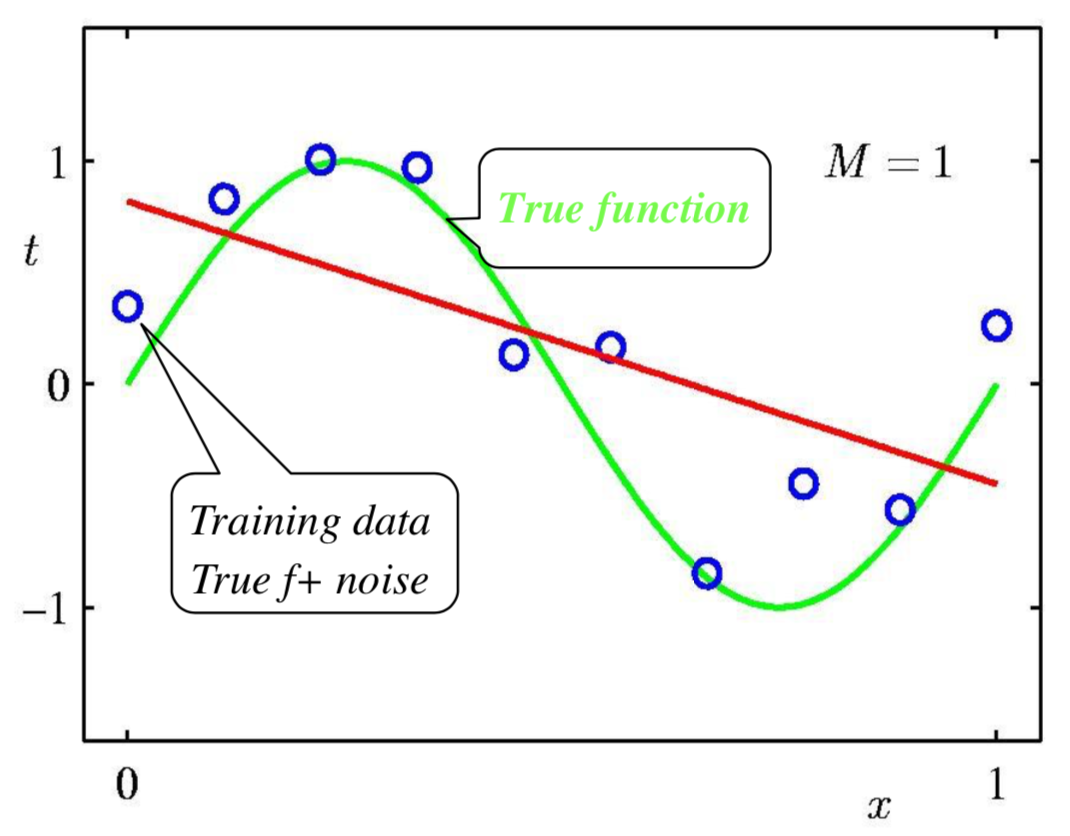
\includegraphics[scale=0.6]{Images/linearnonlinear.png}
\end{figure}

Notiamo che $h_w(X)=w_1x+w_0$ definita "lineare" non significa che é una linea retta, ma piuttosto come il modo in cui i coefficienti w occorrono nell'equazione di regressione (cioè lineare in w, non in x). Quindi, possiamo anche trasformare gli input, come $x,x^2,x^3,...$ con relazioni non lineari tra input e output. Sfruttando l'algoritmo LMS utilizzato fino ad ora:
\begin{equation}
    y(y,w) = w_0+w_1x+w_2x^2+...+w_Mx^M=\sum_{j = 0}^M w_jx^j
\end{equation}

\subsubsection{Esempio}
In LMS la funzione non deve essere lineare nell'argomento (variabili in input) ma solo nei parametri che sono determinati per dare il miglior fit. 
\begin{figure}[H]
    \centering
    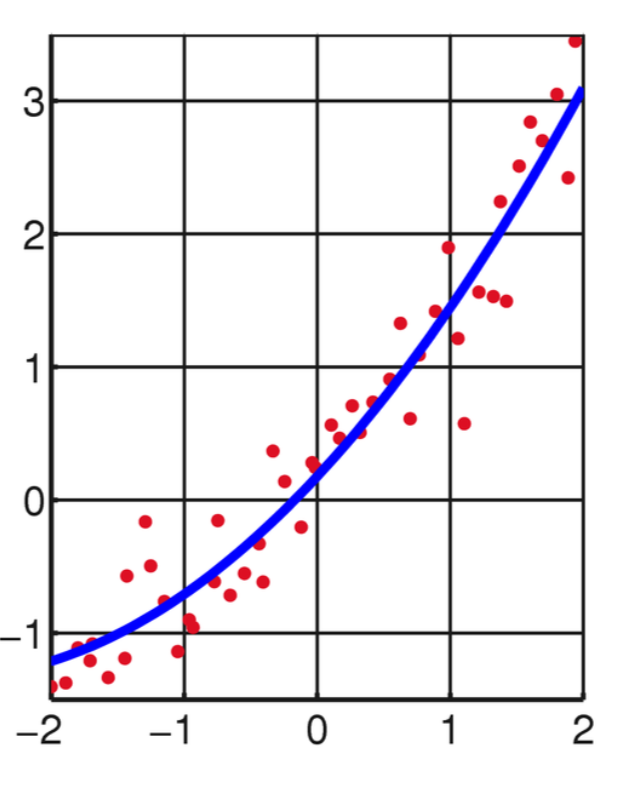
\includegraphics[scale=0.6]{Images/quadraticfit.png}
    \caption{fitting su una funzione quadratica (linea blu) attraverso un set di dati (punti rossi)}
\end{figure}

\subsection{Generalizzazione}
Trasformazione base: linear basis expansion, prima era il prodotto scalare tra w e x (w trasposto per x) ora prendo delle trasformazioni (anche non lineari) del vettore x e le uso come un'espansione della base, combinandole in maniera lineare. 
\begin{equation}
    h_w(x)=\sum_{k=0}^K w_k \phi_k(x)
\end{equation}
Aumenta il vettore di input con variabili aggiuntive che sono trasformazioni di x secondo una funzione phi, ad esempio rappresentazioni polinomiali del tipo $\phi(x)=x_j^2$ oppure $\phi(x)=x_j*x_i$, o ancora trasformazioni non lineari come $\phi(x)=log(x_j)$. Ora il numero dei parametri é $K>n$ soprattutto ora il modello é lineare nei parametri quindi possiamo usare lo stesso algoritmo di prima. 
\subsubsection{Esempi}
\begin{itemize}
    \item dimensione di x=1 $\phi_j(x)=x^j$ 
    \begin{equation}
    h(x) = w_0+w_1x+w_2x^2+...+w_Mx^M=\sum_{j = 0}^M w_jx^j
    \end{equation}
    regressione polinomiale ad 1 dimensione (K=M)
    \item $\phi(x)=\phi([x_1,x_2,x_3]$
    \begin{equation}
    h(x) = w_1x_1+w_2x_2+w_3log(x_2)+w_4log(x_3)+w_5(x_2x_3)+w_0
    \end{equation}
\end{itemize}
quale $\phi$ scegliere? Adottiamo un modello in stile dizioanrio? I punti a favore sono la maggiore espressività poiché può modellare relazioni più complesse di quelle lineari. I punti contro sono l'avere una grossa base di funzioni che richiedono metodi per controllare la complessità del modello, vediamo perché...
\begin{itemize}
    \item grado del polinomio = 1, notiamo che é esegue troppo "underfitting"
    \begin{figure}[H]
    \centering
    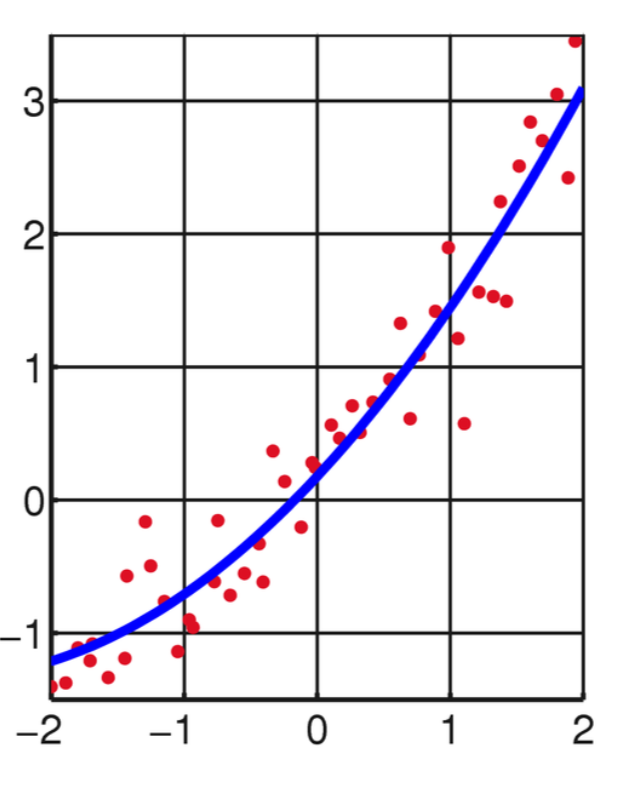
\includegraphics[scale=0.3]{Images/quadraticfit.png}
    \end{figure}
    
    \item ordine del polinomio = 3, notiamo che abbiamo molta più flessibilità ma usciamo dal modello con variabili lineari.
    \begin{figure}[H]
    \centering
    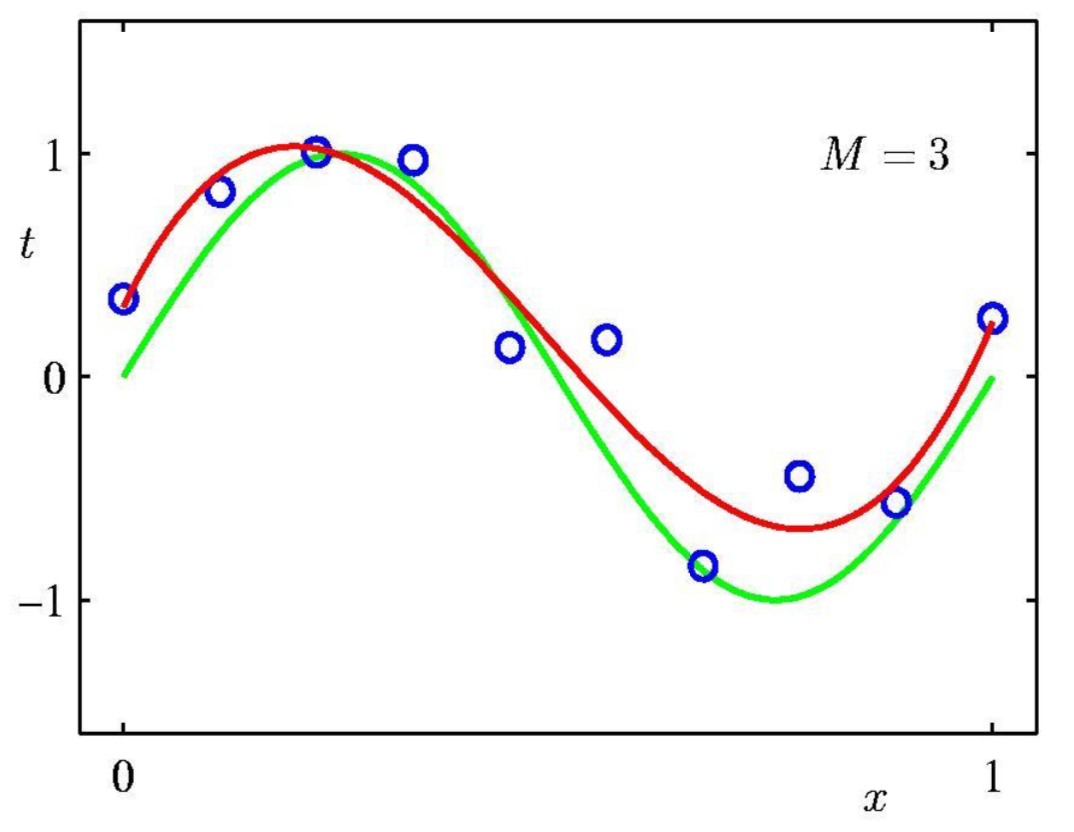
\includegraphics[scale=0.3]{Images/3gradepol.png}
    \end{figure}
    
    \item grado del polinomio = 9, notiamo che é flessibilissimo ma é eccessivo, cioé E(w)=0 ma dobbiamo tenere conto degli errori sul test set, perché se i dati fossero rumorosi noi stiamo "fittando" il rumore.
    \begin{figure}[H]
    \centering
    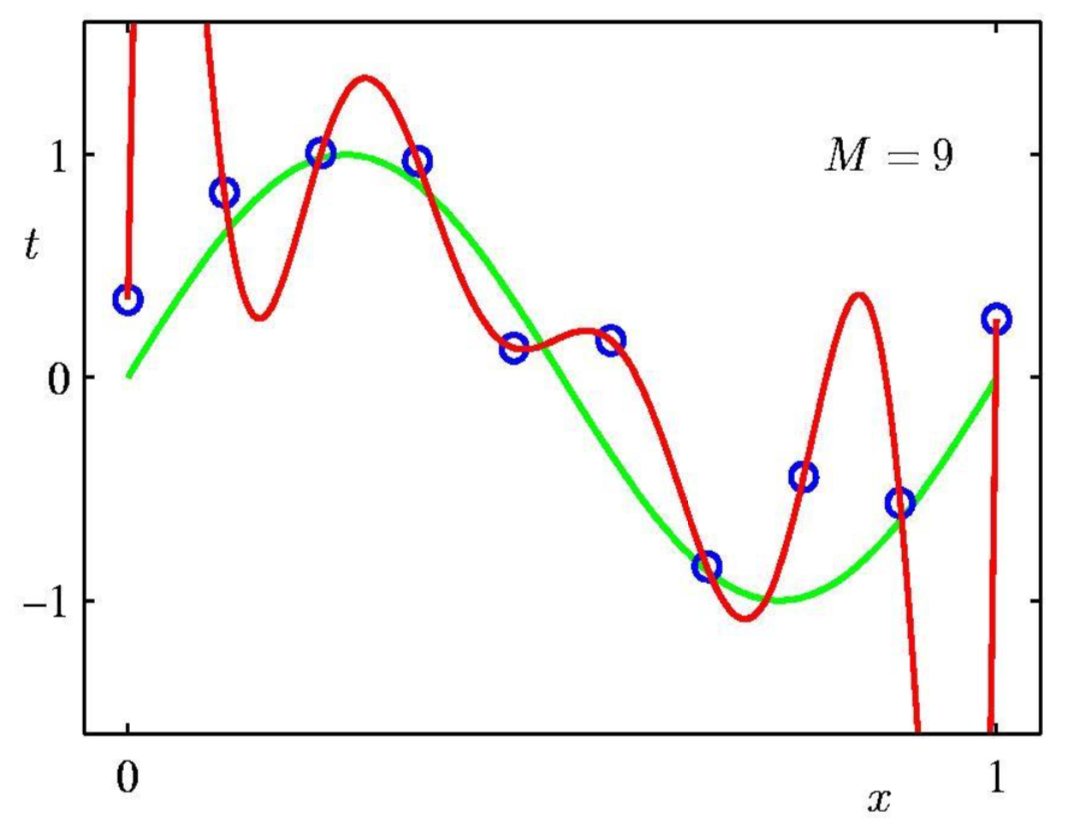
\includegraphics[scale=0.3]{Images/9gradepol.png}
    \end{figure}
\end{itemize}

\subsubsection{Tradeoff per la complessitá}
\begin{itemize}
    \item Se scegliamo un modello troppo semplice non fitta bene i dati e abbiamo una soluzione vincolata (ce ne accorgiamo perché l'errore W è alto) $\rightarrow$ Underfitting
    \item Se scegliamo un modello troppo complesso siamo troppo sensibili alla piccole perturbazioni dei dati $\rightarrow$ Overfitting
\end{itemize}
Vogliamo scegliere la regolarizzazione per bilanciare bias e varianza e lo faremo attraverso il controllo della complessità del modello.
 
\subsection{Verso la regolarizazione}
Possiamo evitare l'overfitting penalizzando le funzioni complicate mantenendo la flessibilitá dello spazio delle ipotesi (un po' come il rasoio di ockham, si preferisce lo spazio delle ipotesi piú semplice che fitta i dati)
\subsubsection{Regolarizzazione Ridge Regression} 
Chiamata anche regolarizzazione di Tikhonov é sempre un modello LMS ma regolarizzato. Per esempio é possibile aggiungere vincoli alla somma del valore di $|w_j|$ favorendo modelli "sparsi", con meno termini dovuti a pesi $w_j$ = 0 (ovvero soluzioni meno complesse). Un modello non regolarizzato fitta bene ma generalizza male (non ci serve a niente). Vorrei un modello semplice (magari con alcuni coefficienti che valgono zero) Come si fa? Aggiungiamo una penalizzazione alla complessità del modello della loss, sommando la norma del vettore w, moltiplicato per un parametro lambda chiamato coefficiente di regolarizzazione. Con il parametro lambda (che é una costante), non ho più bisogno di modificare il grado dei polinomi, o ancora peggio analizzare funzioni più complesse.
\begin{equation}
    definito \quad E_D(w)+\lambda E_W(w) \quad otteniamo \quad Loss(h_w)=\sum_{p} (y_p-h_w(x_p))^2+\lambda ||w||^2
\end{equation}
Ottenendo quindi la nuova regola di apprendimento caratterizzata dal weight decay (aggiunta di $2\lambda w$
\begin{equation}
    w_{new}= w_{old} + \eta*\Delta w - 2 \lambda w_{old}
\end{equation}
Per via di di $-2\lambda w_{old}$ decremento il parametro se positivo, lo incremento se negativo (in pratica lo avvicino a zero $\rightarrow$ weight decay). \newline
Finora abbiamo posto tutta la complessità nel bias di linguaggio, cioè un vincolo posto sul modello (lineare, quadratico, etc). Con la regolarizzazione sposto tutto sul bias di ricerca, cioè sull'algoritmo, come l'algoritmo va a trovare la soluzione (ed è sempre una buona idea). Noi non poniamo a priori una complessità al modello, ma sarà il mio metodo di ricerca intelligente a scegliere la funzione più semplice.
\begin{figure}[H]
\centering
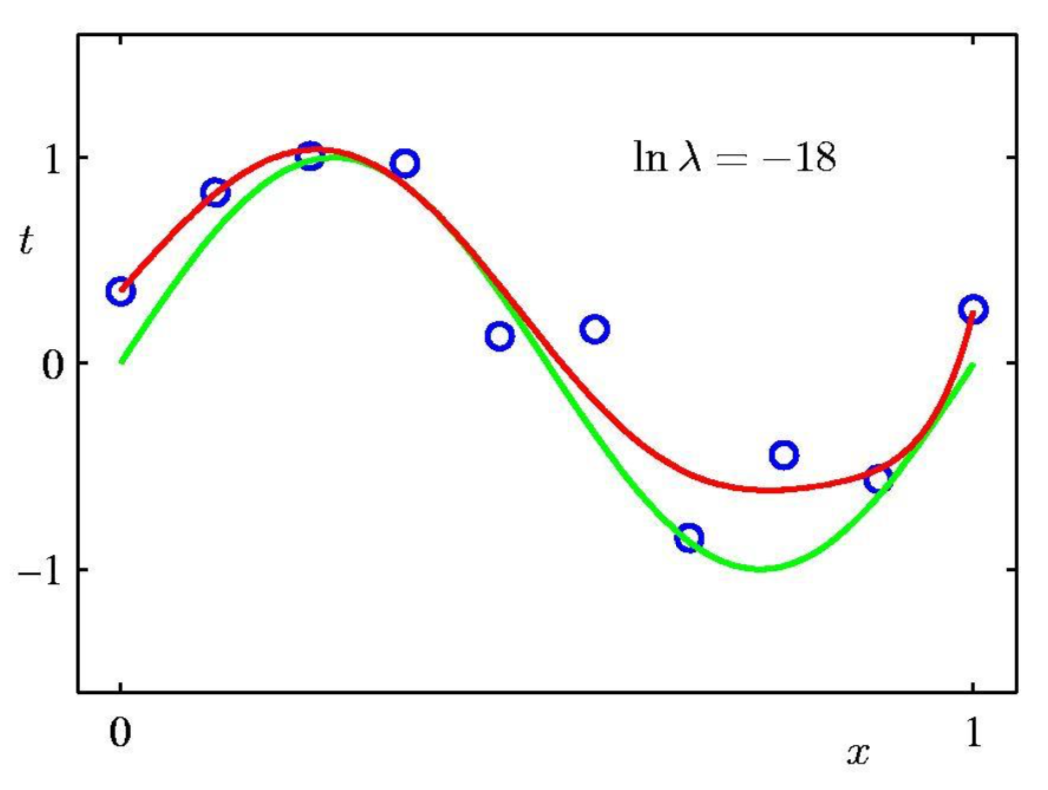
\includegraphics[scale=0.3]{Images/9gradopollambda.png}
\caption{Polinomio di grado 9 con $log_e(\lambda) = -18$ quindi $\lambda$ basso}
\end{figure}

\begin{figure}[H]
\centering
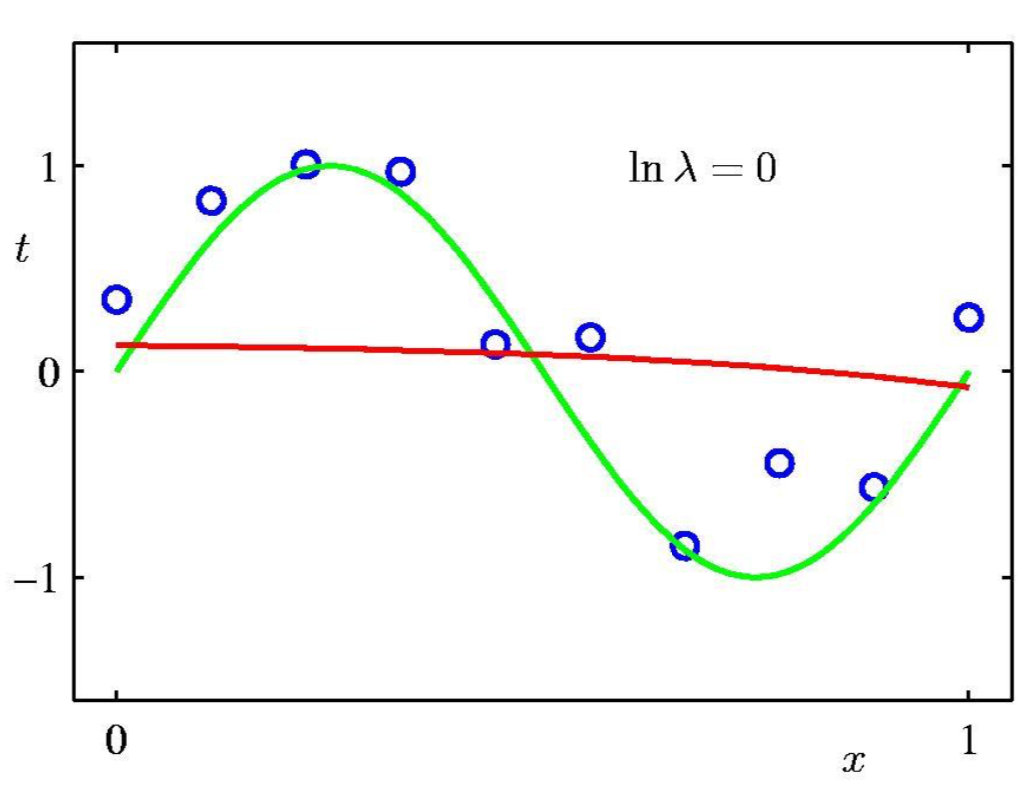
\includegraphics[scale=0.3]{Images/9gradopollambda0.png}
\caption{Polinomio di grado 9 con $log_e(\lambda) = 0$ quindi $\lambda$ tropo alto}
\end{figure}

\begin{figure}[H]
\centering
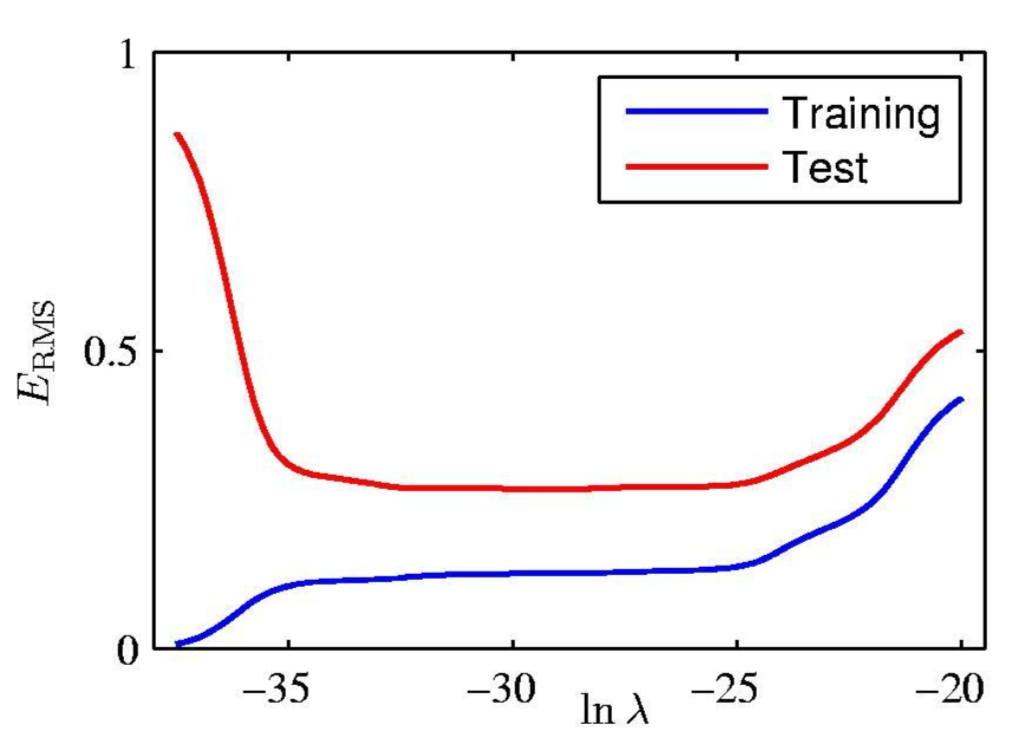
\includegraphics[scale=0.3]{Images/Ermsvslambda.png}
\caption{$E_{RMS}$ vs $log_e(\lambda)$}
\end{figure}

Possiamo concludere quindi dicendo che se $\lambda$ é basso $\rightarrow$ overfitting, mentre se $\lambda$ alto $\rightarrow$ underfitting.

\subsection{Limitazione delle funzioni a base fissa}
Quando facciamo un'espansione polinomiale, la dimensionalità del problema cresce molto, e i dati che prima erano densi, potrebbero diventare sparsi. Quando la dimensione dell'input aumenta, il problema diventa enormemente difficile (la difficoltà cresce esponenzialmente, proprio come il volume con le dimensioni). Inoltre, se inizio a mettere dati a caso, rischio di aumentare il rumore. Avere la funzione base che opera su ogni dimensione di uno spazio implica che lo spazio di input richieda un numero combinatorio di funzioni. Per esempio un polinomio dell'ordine 3, utilizza tutte le combinazioni di variabili di input dovute ai prodotti $x_1x_2, x_2x_3, ..., x_1x_2x_3 ecc. \rightarrow D^3$ (approssimazione come aumento D) \newline
In altri modelli, vedremo come possiamo farcela con meno funzioni di base. Si sceglie il test dizionario e si mettono dei parametri liberi, per adattare la phi ad H.
Ho il vantaggio di essere più generale, ma il modello diventa non lineare rispetto a w (reti neurali). \newline 
In altri modelli invece di calcolare esplicitamente la phi, viene fatta in maniera implicita, col concetto di kernel, controllando il modello direttamente con la funzione obiettivo, non più con una penalità aggiunta dopo (SVM).

\subsection{Classificazione con il modello lineare}
Possiamo utilizzare il modello lineare per la classificazione, in questo caso usiamo un iperpiano (wx) assumento valori positivi o negativi. Sfruttiamo questi modelli per decidere se un punto x appartiene alla zona positiva o negativa dell'iperpiano. Quindi vogliamo impostare w (imparando) in mod tale da ottenere una buona precisione di classificazione.
\subsubsection{Visione geometrica dell'iperpiano}
$w^Tx$ definisce un iperpiano, il decision bundary é il luogo geometrico dei punti dove l'iperpiano (il prodotto scalare) vale zero e puó essere utilizzator per classificare.
\begin{figure}[H]
\centering
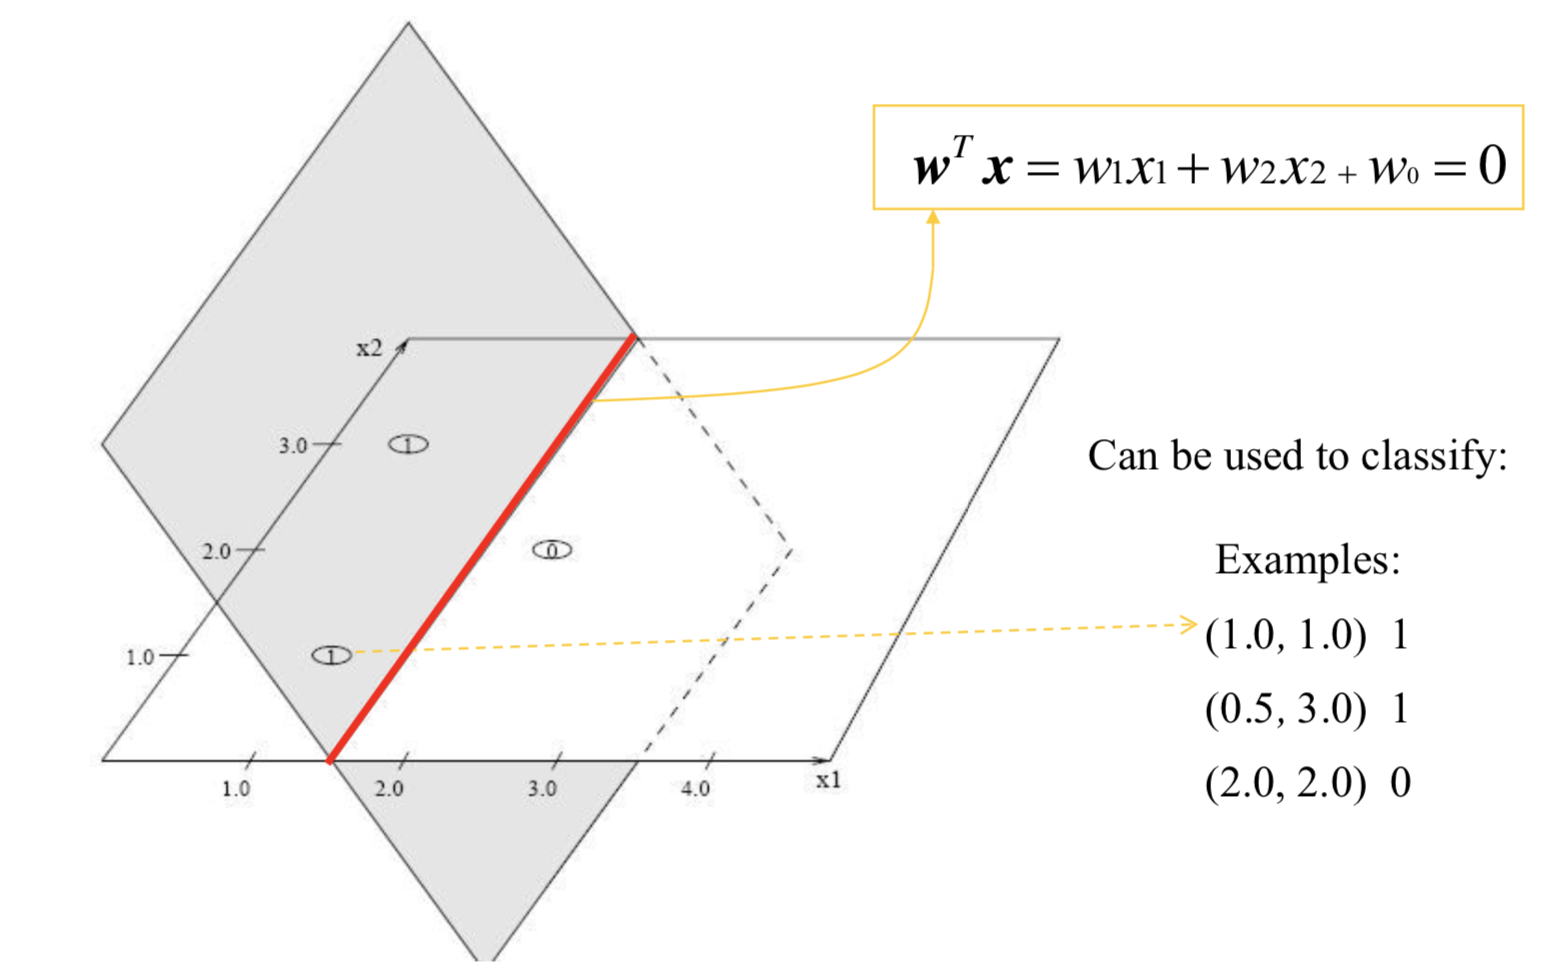
\includegraphics[scale=0.5]{Images/deecisionbundary.png}
\end{figure}
Quindi possiamo definire una funzione di classificazione del tipo
\begin{equation}
  h(x)=\begin{cases}
    1 & \text{if $wx+w_0\geq 0$}.\\
    0 & \text{altrimenti}.
  \end{cases}
\end{equation}
che possiamo scrvere come $h(x)=sign(wx+w_0)$ $\rightarrow$ $h(x_p)=sign(x_p^Tw)=sign(\sum_{i=0}^n x_{p,i}w_i)$
\begin{figure}[H]
\centering
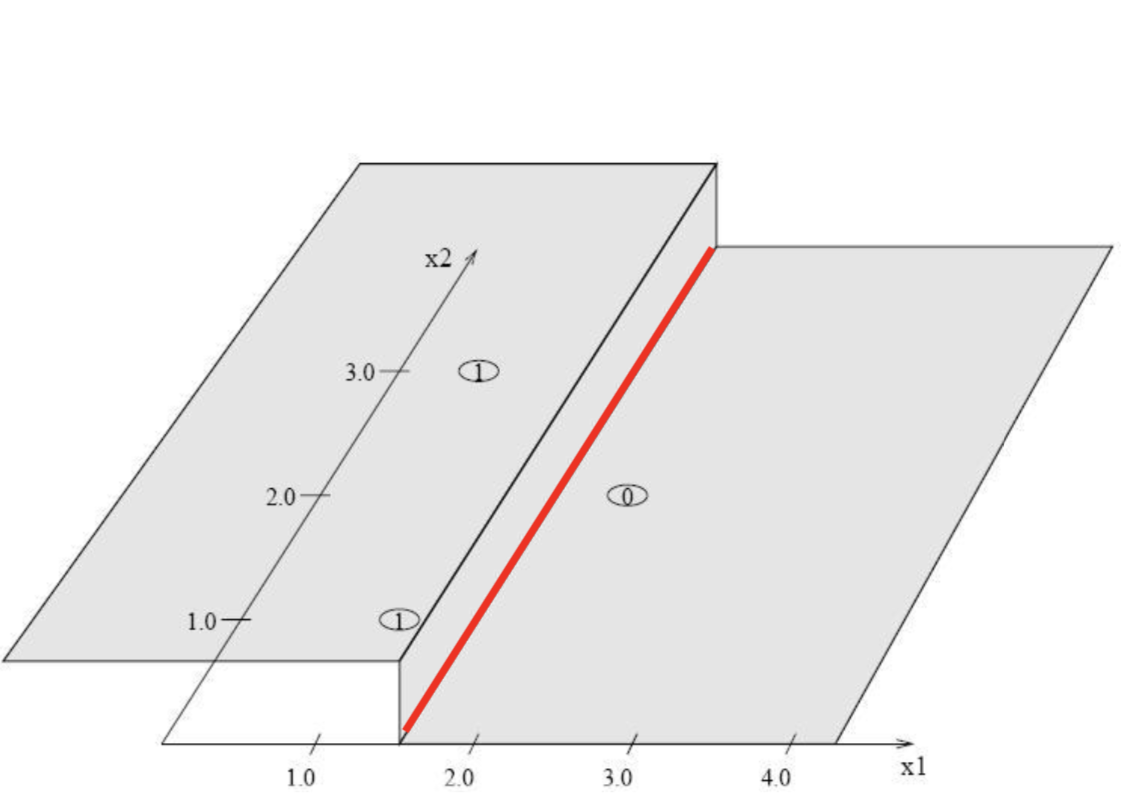
\includegraphics[scale=0.5]{Images/classificationplane.png}
\end{figure}

\subsubsection{Classificazione attraverso decision boundary lineare}
La classificazione puó essere vista come come l'allocazione dello spazio in input in diverse regioni di decisione. Ad esempio in uno spazio di due dimensioni $x=(x_1,x_2)$ in $R^2$ e $f(x)=0 \lor 1$. In questo caso non vedremo il piano separatore, vediamo solo wx = 0. \begin{quote}
    Linear Threshold unit (LTU) = Indicatore di funzioni, quanti ne abbiamo? un insieme di dicotomie indotte da iperpiani, sono tutti i modi che abbiamo per muovere la linea rossa.
\end{quote}
\begin{figure}[H]
\centering
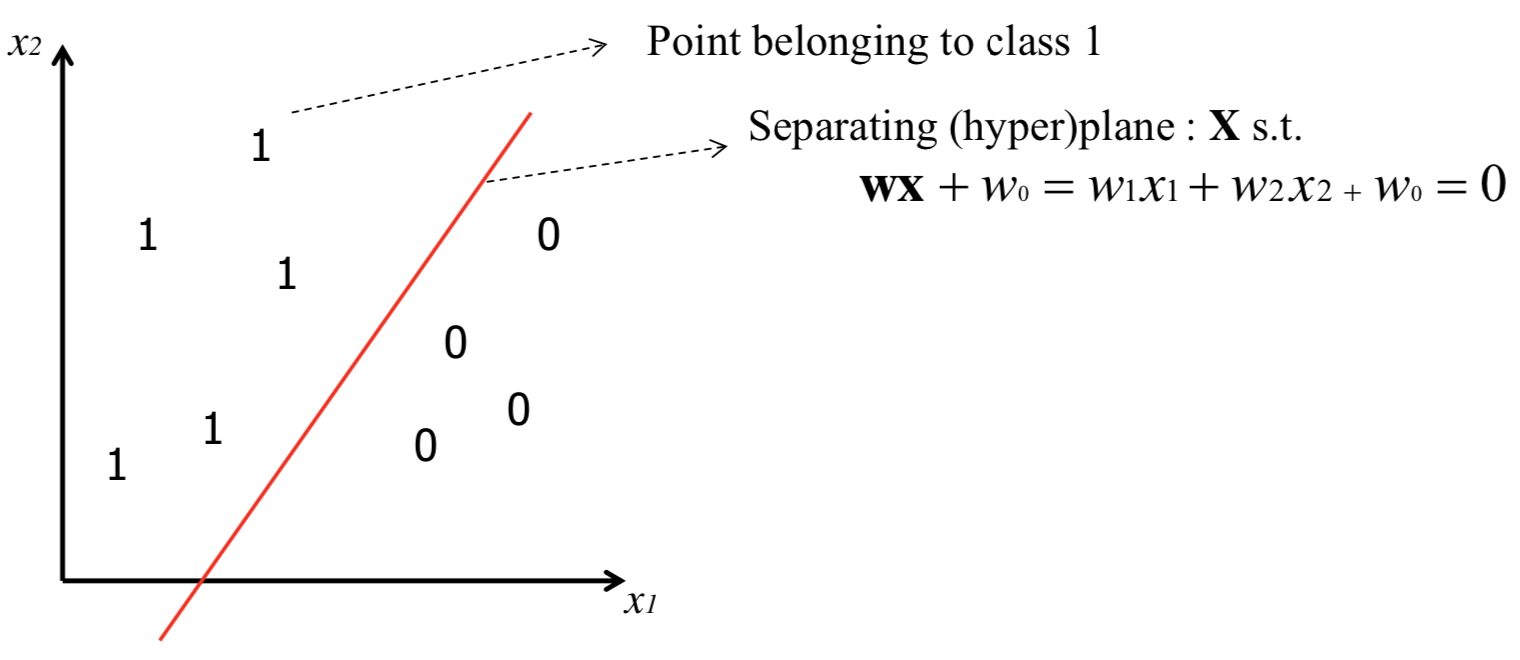
\includegraphics[scale=0.5]{Images/lineardecisionboundary.png}
\end{figure}

\subsubsection{Esempio Terremoti/Esplosioni Nuclerari}
Trovare h in modo tale che il dato (x1, x2) ritorni (0 $\lor$ -1) per i terremoti e (1) per esplosioni nucleari. I dati sismici sono rappresentati da x1 che é la magnitudine dell'onda del corpo e x2 che é la magnitudine dell'onda della superficie. L'algoritmo trova il decision boundary.
\begin{figure}[H]
\centering
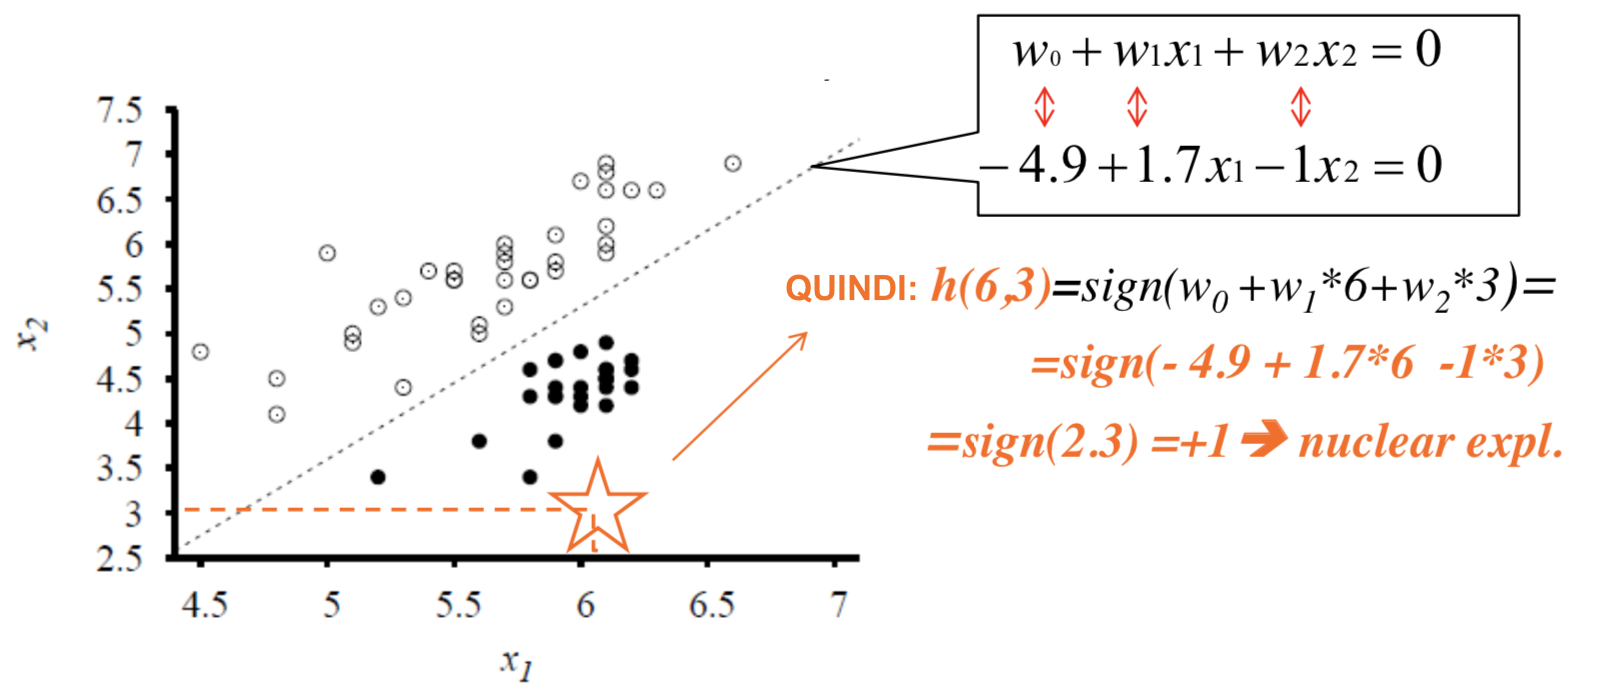
\includegraphics[scale=0.5]{Images/magnitudegraph.png}
\end{figure}

\subsubsection{Esempio Email Spam}
Trovare h(mail) in modo tale che resistuisca +1 se é spam e -1 se non é una mail spam. $\phi(mail)$ = parole [0/1] o frasi (“denaro gratis”)
[0/1] o lunghezza [intero], ad esempio $\phi_k(x)=contain(word_k)$ e w peso per le le funzioni di input che aiutano alla previsione, cioé peso positivo per "denaro gratis", negativo per ".edu". wx é la combinazione del peso. $h_w(x)$ provvede a dare il limite per decidere se una mail é spam o non é spam.
\begin{equation}
    h_w(x)= segno(\sum_{k} w_k\phi_k(x))
\end{equation}

\subsubsection{Il problema di apprendimento (per classificatori lineari)}
Assumendo che usiamo ancora il metod dei minini quadrati, dato un insieme di esempi di allenamento l bisogna trovare w che minimizza la somma residua dei quadrati
\begin{equation}
    E(w)=\sum_{p\rightarrow l}(y_p-x_p^Tw)^2=||y-Xw||^2
\end{equation}
L'errore minimo: se $y_p=1$ allora $x_p^Tw \rightarrow 1$ mentre se $y_p=0\lor -1$ allora $x_p^Tw \rightarrow 0 \lor -1$. NOTA: in E(w) non usiamo la forma h(x) come per la regressione, per contenere una perdita continua differenziabile perché usiamo h(x)=segno(wx) per la classificazione. Abbiamo ancora l'algoritmo di discesa del gradiente:
\begin{equation}
    \Delta w_i = - \frac{\partial E(w)}{\partial w_i} = \sum_{p=1}^l (y_p - (x_p^Tw)) * x_{p,i}
\end{equation}
Nella derivata ignoriamo il 2 che viene fuori dal quadrato. È una costante che non incide sull'eta (il coefficiente di apprendimento).

\subsubsection{$\Delta w$ come regola della correzione dell'errore}
Se un input viene classificato erroneamente, quindi il Delta positivo per $w_1$ e $w_3$, bisogna aumentare $w_1$ e $w_3$ proporzionalmente (con eta) al delta, quindi un valore positivo in questo caso. Correzione d'errore: alzo i valori dove sono troppo bassi, e viceversa.
\begin{figure}[H]
\centering
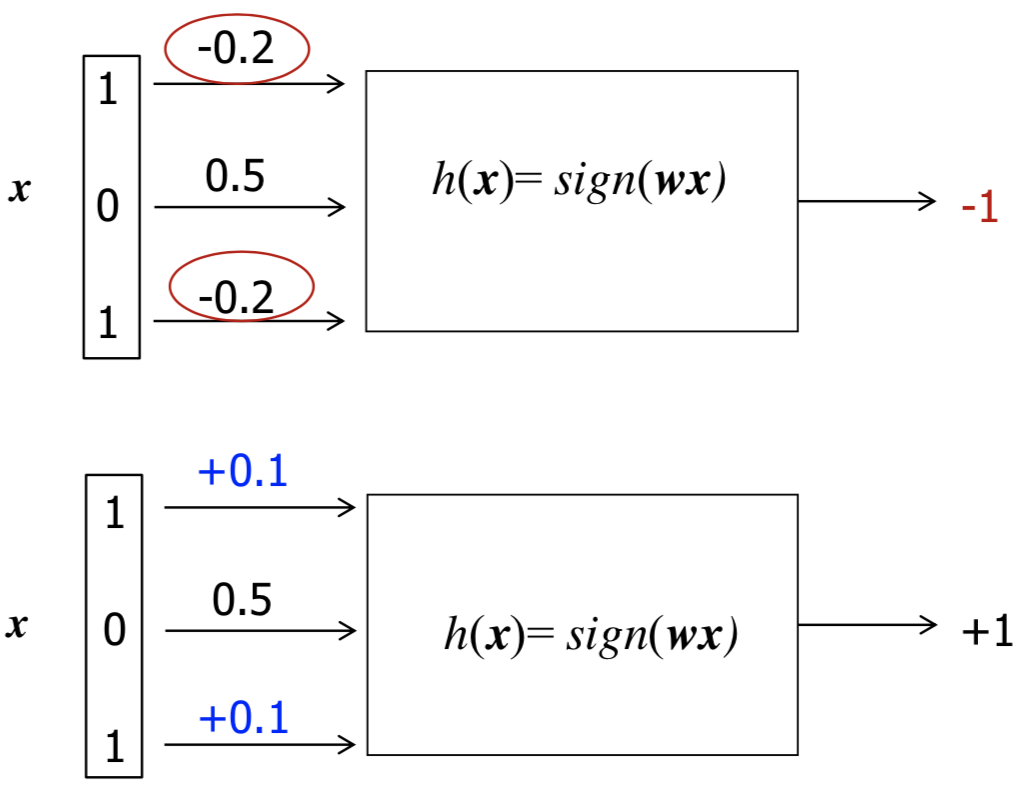
\includegraphics[scale=0.5]{Images/errorcorrection.png}
\end{figure}

\subsection{Riassunto}
Il modello viene allenato su un insieme di esempi con LMS su wx dall'algoritmo di discesa del gradiente usato per la regressione lineare. Il modello viene usato per la classificazione applicando la funzione di soglia $h(x)=segno(wx)$. L'errore puó essere calcolato come errore di classificazione o numero di pattern classificati erroneamente. 
\begin{equation}
  L(h(x_p),d_p)=\begin{cases}
    0 & \text{se $h(x_p)=d_p$}.\\
    1 & \text{altrimenti}.
  \end{cases}
  \quad mean_err = \frac{1}{l\sum_{i=1}^l L(h(x_i), d_i)}
\end{equation}
\begin{quote}
    Accuratezza = media dei pattern correttamente classificati = $(l-numerr)/l$ \newline dove $numerr=\sum_{i=1}^l L(h(x_i), d_i)$
\end{quote}
\subsection{Learning Algorithm}
É lo stesso come per la regressione $\rightarrow$ Algoritmo gradiente discendente (anche l'espansione lineare e Tikhonov possono essere applicati). Notare che l'algortimo converge asintoticamente al MinLeastSqaure, non necessariamente al numero minimo di errori di classificazione. Perché nella loss non ha il numero di errori di classificazione. Bisogna tener conto di quello che fanno davvero gli algoritmi, e non di quello che vorremmo che facessero (anche se ci sono algorirmi che minimizzano gli errori di classificazione)
\subsubsection{Congiunzioni nel caso di modello lineare}
Possiamo rappresentare congiunzioni tramite un modello lineare ad esempio:\newline
$x_1 \land x_2 \land x_4 \Leftrightarrow y$ cioé $1x_1+1x_2+0x_3+1x_4 > 2$ oppure $1x_1+1x_2+0x_3+1x_4 > 2.5$ \newline
altro esempio: \newline
$x_1 \land x_2$ cioé $1x_1+1x_2>1$ oppure $1x_1+1x_2>1.5$ 
\begin{figure}[H]
\centering
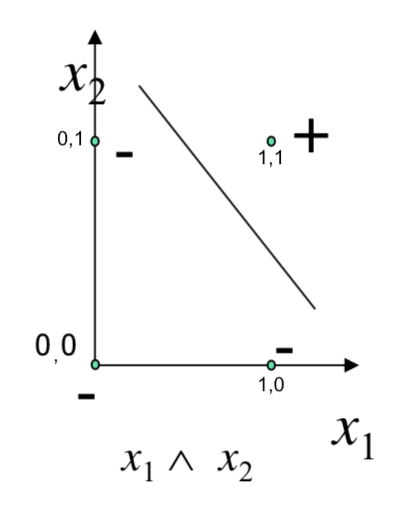
\includegraphics[scale=0.5]{Images/conjunctionsgraph.png}
\end{figure}
in generale w puó essere appreso per trovare la soluzione. 
\subsubsection{Limitazioni}
Nella geometria due insiemi di punti in un grafico a due dimensioni  sono linearmente separabili quando il due insiemi di punto possono esser separati da una singola linea. In generale due gruppi di punti sono linearmente separabili in uno spazio di dimensione n se possono essere separati da un iperpiano di dimensione n-1. Il confine lineare provvede la soluzione esatta solo per insiemi di punti linearmente separabili. 

\begin{figure}[H]
\centering
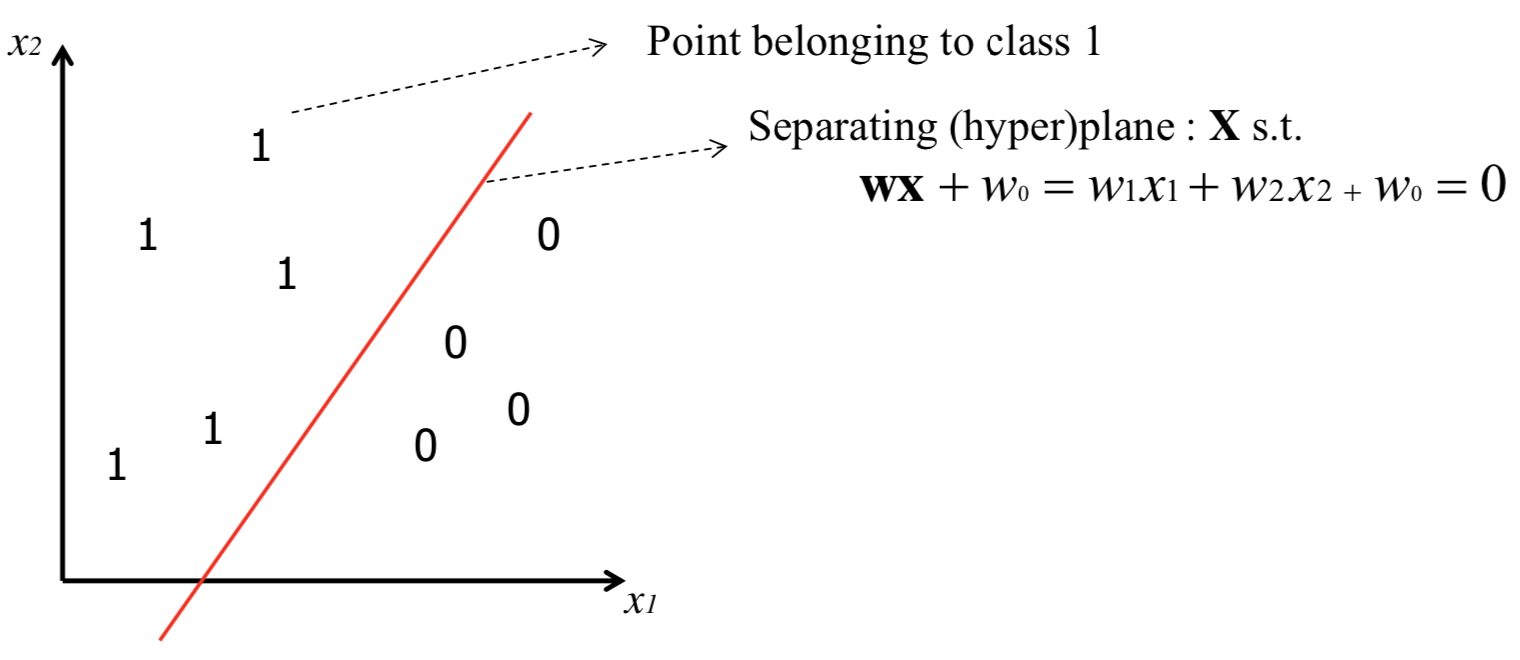
\includegraphics[scale=0.5]{Images/lineardecisionboundary.png}
\end{figure}

\subsection{Altri sistemi di apprendimento per la classificazione}
\begin{itemize}
    \item Linear Discriminant Analysis
    \item Logistic Regression: Stima la/le proprietà di x dato y, P(y/x) partendo modellando la densitá della classe come densitá nota. Abbiamo una soglia soft (continua, differenziabile) con funzione logica (anziché soglia hard 0/1)
    \item Reti Neurali e SVM: modelli flessibili che includono approssimazione non lineare sia per la regressione che per la classificazione.
\end{itemize}

\subsection{Conclusioni}
I modelli lineari sono un approccio fondato di base per la regressione e la classificazione, é un modo molto compatto per rappresentare la conoscenza (tutti i dati sono in w) ma con una forte assunzione sulla relazione tra i dati (Assumiamo che ci sia una relazione lineare tra i dati, o comunque in accordo alla phi che abbiamo scelto; è un'assunzione molto forte sullo spazio delle ipotesi). Abbiamo visto un algoritmo di correzione iterativa dell'errore (LMS) che ricerca spazi di ipotesi continui, una visione dei limiti ad approcci lineari e delle esigenze per modelli di ML più flessibili e anche i loro problemi: Un'estensione del modello lineare per attività non lineari e un'introduzione al controllo della complessità (regolarizzazione).


















%\bibliographystyle{plain}
%\bibliography{references}
\end{document}
